% =================================================================================================
% File:     server_tier/processor.tex
% Description:  Definisce la sezione relativa al back-end dell'applicazione
% Created:    2015-04-07
% Author:   Cusinato Giacomo
% Email:    cusinato.giacomo@mashup-unipd.it
% =================================================================================================
% Modification History:
% Version   Modifier Date   Change                      Author
% 0.0.1
% =================================================================================================

% CONTENUTO DEL CAPITOLO


\subsubsection{server::processor} % (fold)
\label{ssub:bdsm_app_server_processor}
\begin{figure}[!htbp]
  \centering
  \centerline{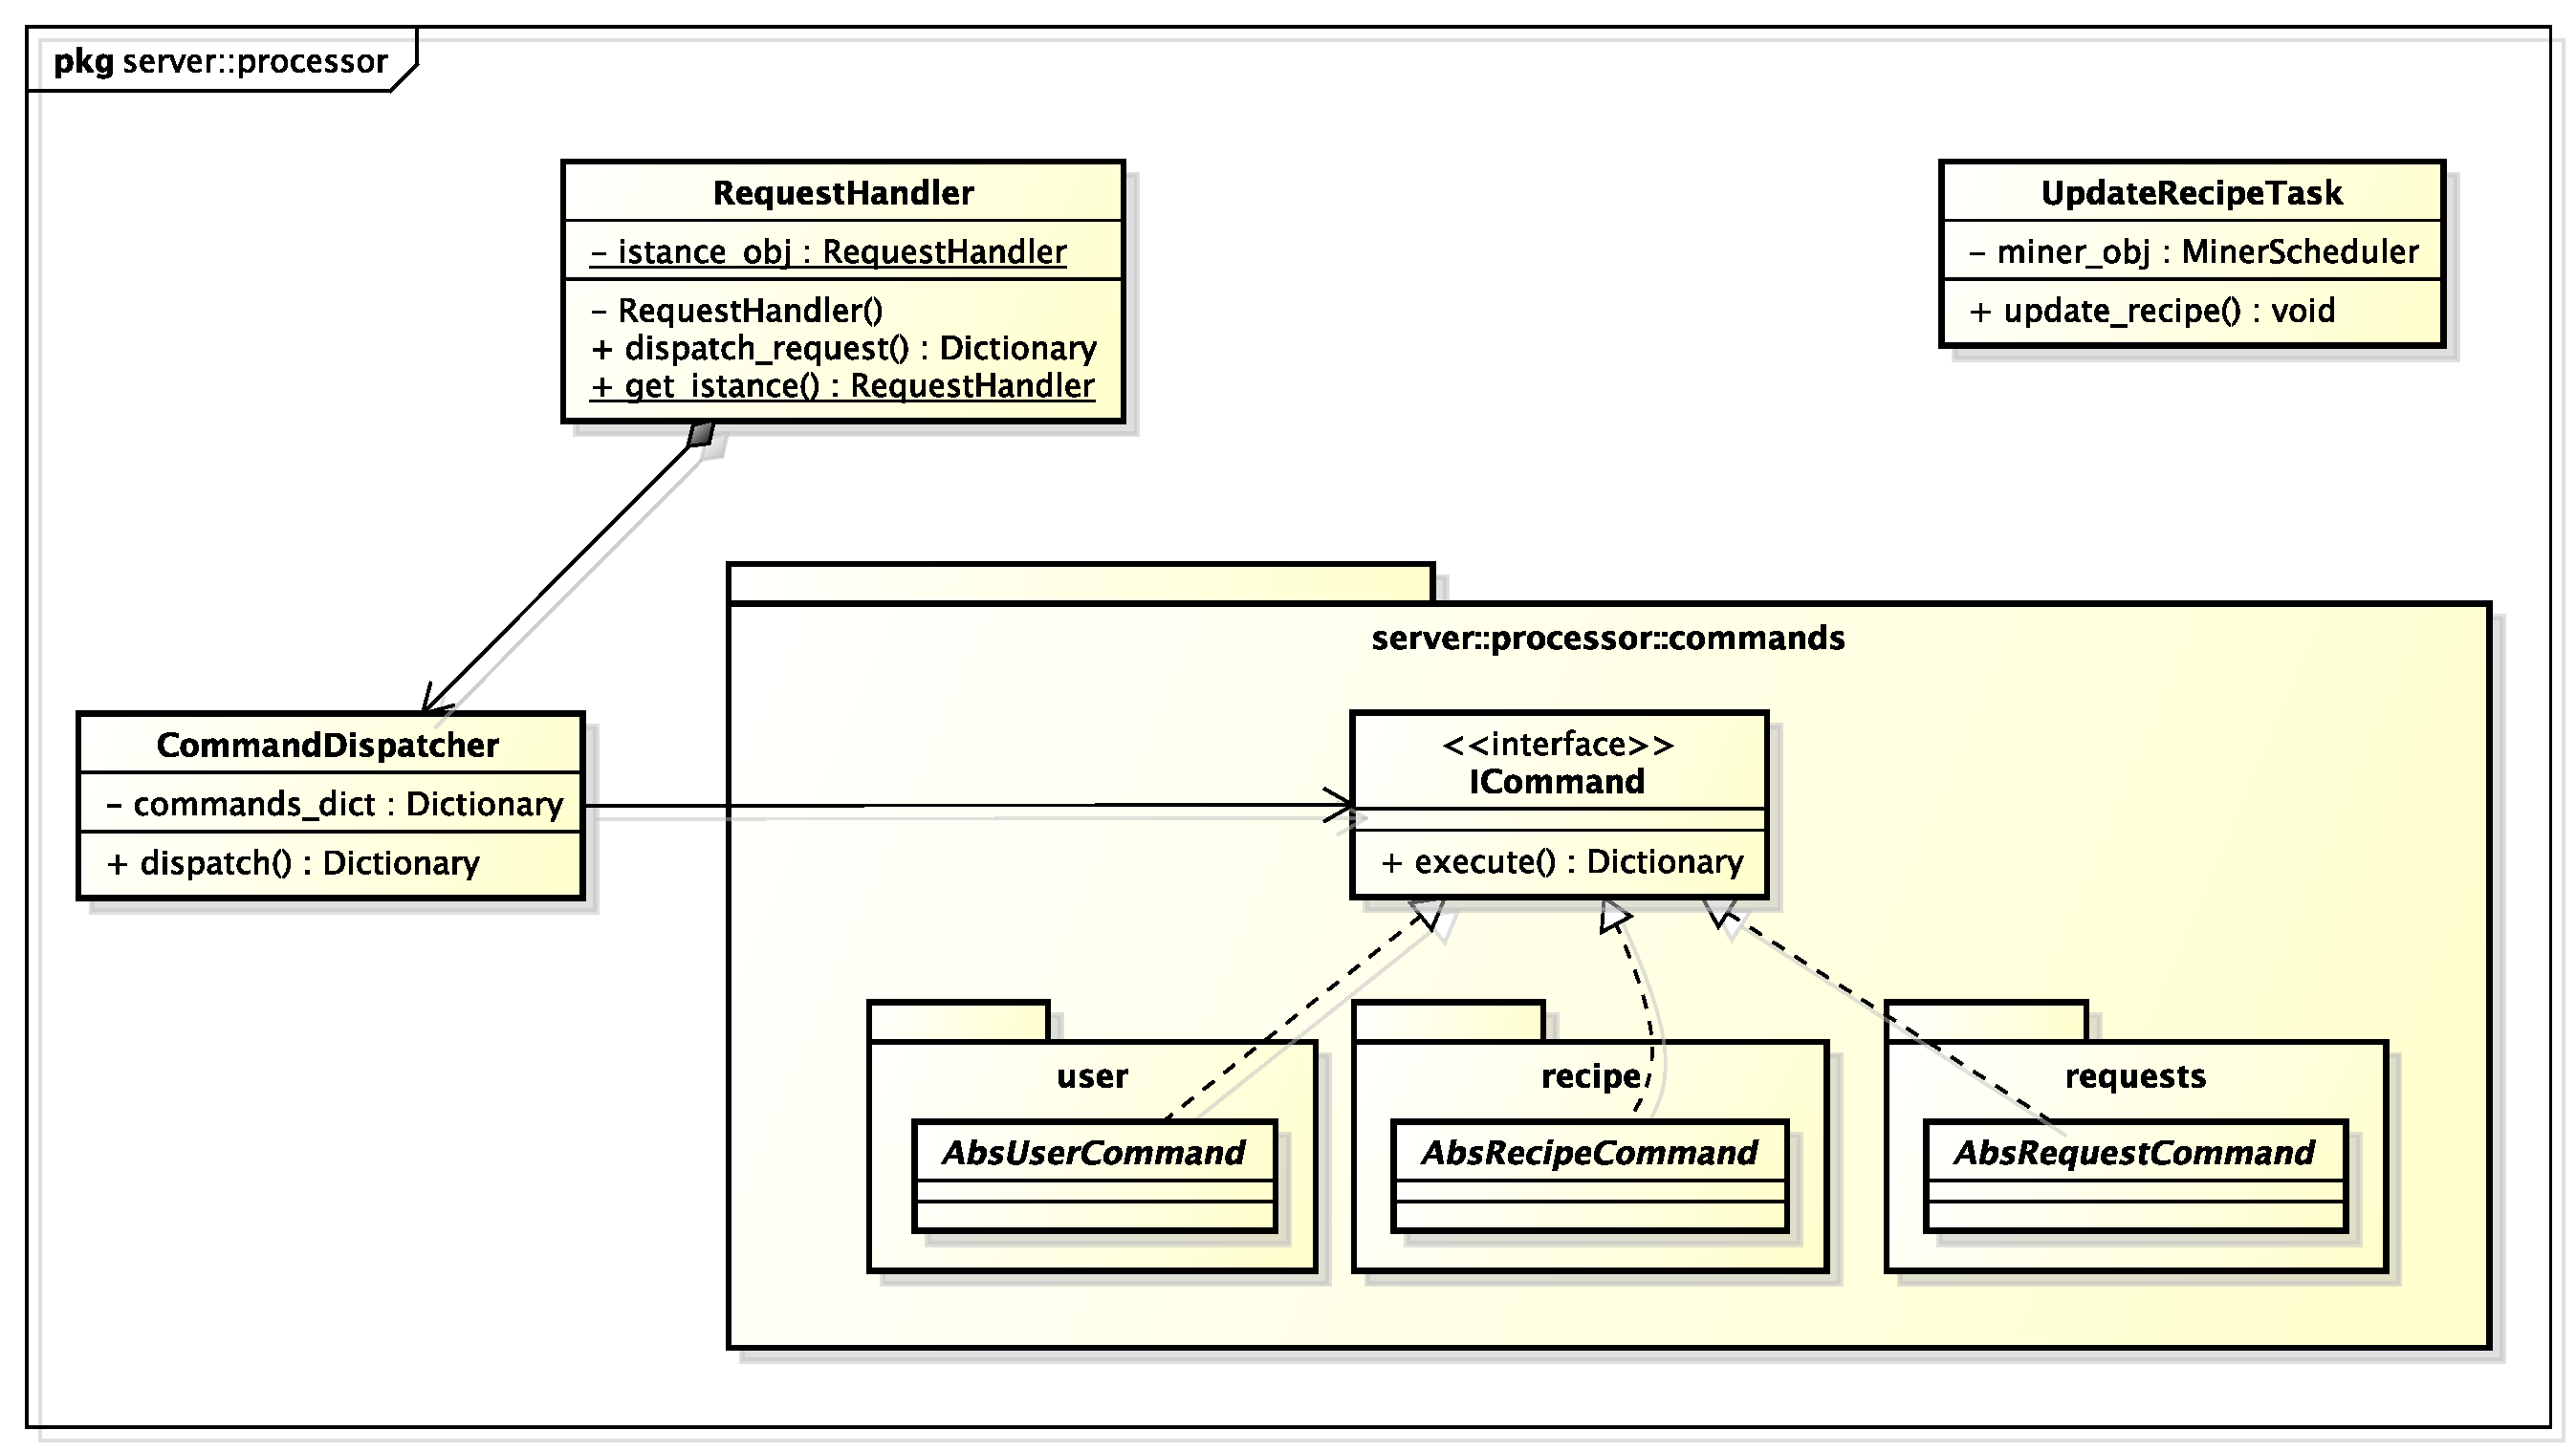
\includegraphics[scale=0.4]{./images/server/processor.pdf}}
  \caption{Package - server::processor}
\end{figure}

\begin{itemize}
  \item \textbf{Descrizione}: è il package che contiene le componenti che gestiscono le richieste in arrivo dal client grazie ai servizi REST definiti nel package \texttt{server::endpoints::api};
  \item \textbf{Padre}: server
  \item \textbf{Package contenuti}: server::processor::commands
  \item \textbf{Interazione con altri componenti}:
    \begin{itemize}
      \item server::miner
      \item server::endpoints
      \item server::db
    \end{itemize}
\end{itemize}

  \paragraph{Classi} % (fold)

\subparagraph{server::processor::RequestHandler} % (fold)
    \label{subp:bdsm_app_server_processor_requesthandler}
    \begin{figure}[!htbp]
  		\centering
 		\centerline{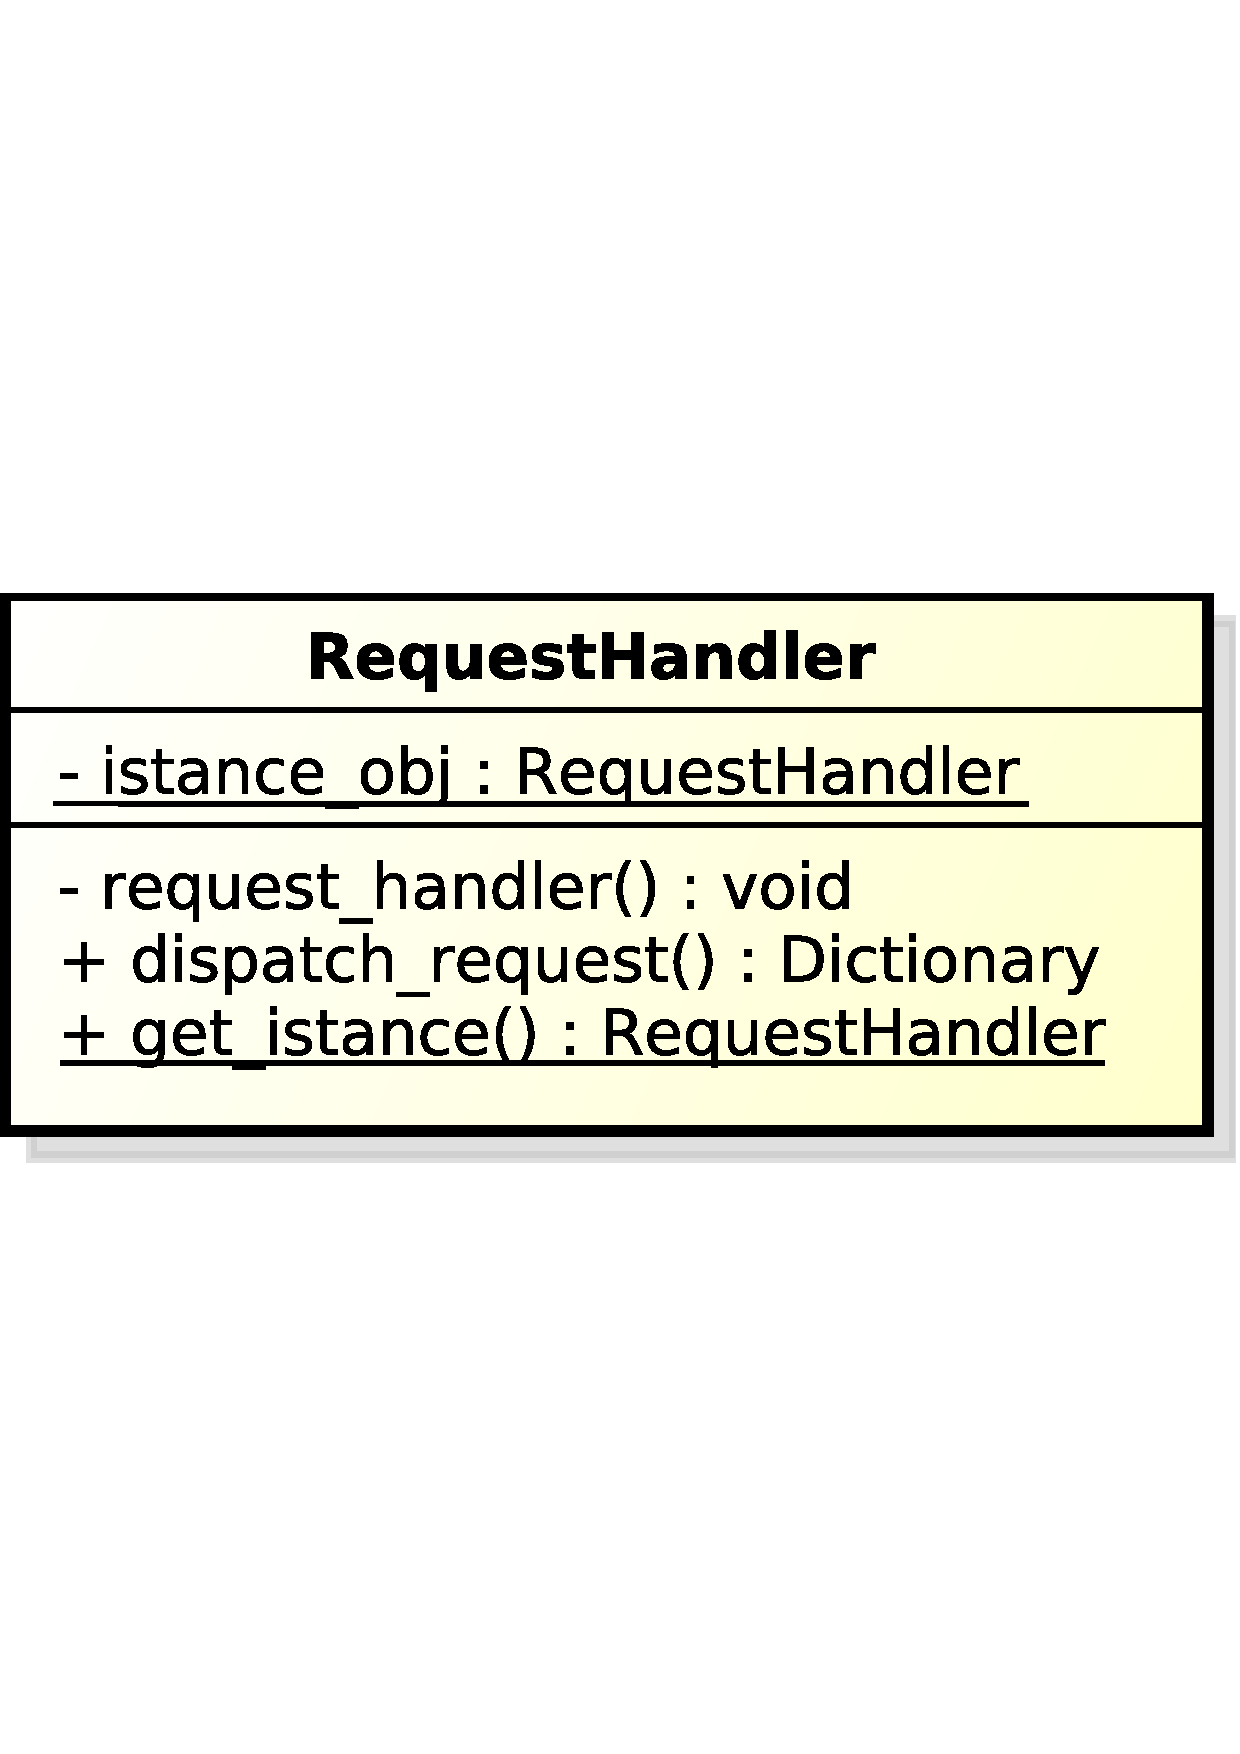
\includegraphics[scale=0.75]{./images/server/classes/processor/request_handler.pdf}}
 		\caption{Classe - server::processor::RequestHandler}
	\end{figure}
    \begin{itemize}
      \item \textbf{Descrizione}: è la classe che implementa il pattern Front Controller e si occupa di raccogliere le richieste provenienti dal client. Implementa inoltre il pattern Singleton, perciò un'unica istanza di tale classe vivrà nel sistema;
      \item \textbf{Utilizzo}: viene invocata dalle classi presenti nel package \texttt{server::endpoints::api} in seguito ad una chiamata ai servizi REST offerti dal sistema e trasferisce la richiesta alla classe \texttt{CommandDispatcher} che si occuperà di invocare il relativo comando per soddisfare tale richiesta;
      \item \textbf{Relazioni con altre classi}:
        \begin{itemize}
          \item server::processor::CommandDispatcher
        \end{itemize}
      \item \textbf{Attributi}:
          \begin{itemize}
              \item \textcolor{forestgreen}{\texttt{- static istance\_obj : RequestHandler}}
              \begin{description}
                \item \textbf{Descrizione}: rappresenta la singola istanza della classe RequestHandler.
              \end{description}
          \end{itemize}
      \item \textbf{Metodi}:
          \begin{itemize}
             \item \textcolor{forestgreen}{\texttt{- request\_handler()}}
              \begin{description}
                \item \textbf{Descrizione}: costruttore privato del singleton RequestHandler.
              \end{description}
             \item \textcolor{forestgreen}{\texttt{+ dispatch\_request(request\_name: String, request\_args: Dictionary) : Dictionary}}
              \begin{description}
                \item \textbf{Descrizione}: metodo che si occupa di far confluire la richiesta in arrivo alla classe CommandDispatcher. I dati della richiesta vengono rappresentati come un dizionario chiave-valore, come quelli della risposta che saranno ritornati al chiamante.
              \end{description}
             \item \textcolor{forestgreen}{\texttt{+ static get\_istance() : RequestHandler}}
              \begin{description}
                \item \textbf{Descrizione}: ritorna la singola istanza della classe RequestHandler o ne crea una se tale classe non risulta ancora istanziata.
              \end{description}
          \end{itemize}
      \end{itemize}
    % subparagraph bdsm_app_server_processor_requesthandler (end)

\subparagraph{server::processor::CommandDispatcher} % (fold)
    \label{subp:bdsm_app_server_:processor_commanddispatcher}
    \begin{figure}[!htbp]
  		\centering
 		\centerline{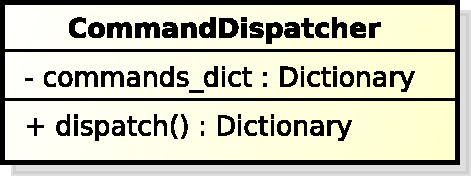
\includegraphics[scale=0.75]{./images/server/classes/processor/command_dispatcher.pdf}}
 		\caption{Classe - server::processor::CommandDispatcher}
	\end{figure}
    \begin{itemize}
      \item \textbf{Descrizione}: classe che implementa il pattern Command e si occupa di far confluire una determinata richiesta al relativo comando contenente la logica per soddisfarla;
      \item \textbf{Utilizzo}: contiene un dizionario che mappa tutte le tipologie di richieste al relativo comando che sarà invocato tramite il metodo \texttt{dispatch()}. Si occupa inoltre di ritornare al Front Controller un dizionario contenente un'eventuale risposta per il client;
      \item \textbf{Relazioni con altre classi}:
        \begin{itemize}
          \item server::processor::commands::ICommand
        \end{itemize}
    \item \textbf{Attributi}:
          \begin{itemize}
              \item \textcolor{forestgreen}{\texttt{- commands\_dict : Dictionary}}
              \begin{description}
                \item \textbf{Descrizione}: contiene una mappa che collega ogni tipologia di richiesta ad un determinato comando. Questo dizionario ci permette di avere una lista completa e ordinata di associazioni tra i metodi delle API e i comandi che devono utilizzare in modo da facilitarci la gestione delle chiamate ai comandi. Una richiesta è rappresentata da una specifica stringa.
              \end{description}
          \end{itemize}
    \item \textbf{Metodi}:
          \begin{itemize}
              \item \textcolor{forestgreen}{\texttt{+ dispatch(request\_name: String, request: Dictionary) : Dictionary}}
              \begin{description}
                \item \textbf{Descrizione}: metodo che si occupa di far confluire un determinata richiesta (ed i dati associati mappati in un dizionario) ad un determinato comando grazie all'attributo \texttt{commands\_dict}. Ritorna la risposta alla chiamata tramite un dizionario.
              \end{description}
          \end{itemize}
      \end{itemize}
    % subparagraph bdsm_app_server_processor_commanddispatcher (end)


    \subsubsection{server::processor::commands} % (fold)
    \label{ssub:bdsm_app_server_processor_commands}
    \begin{figure}[!htbp]
      \centering
      \centerline{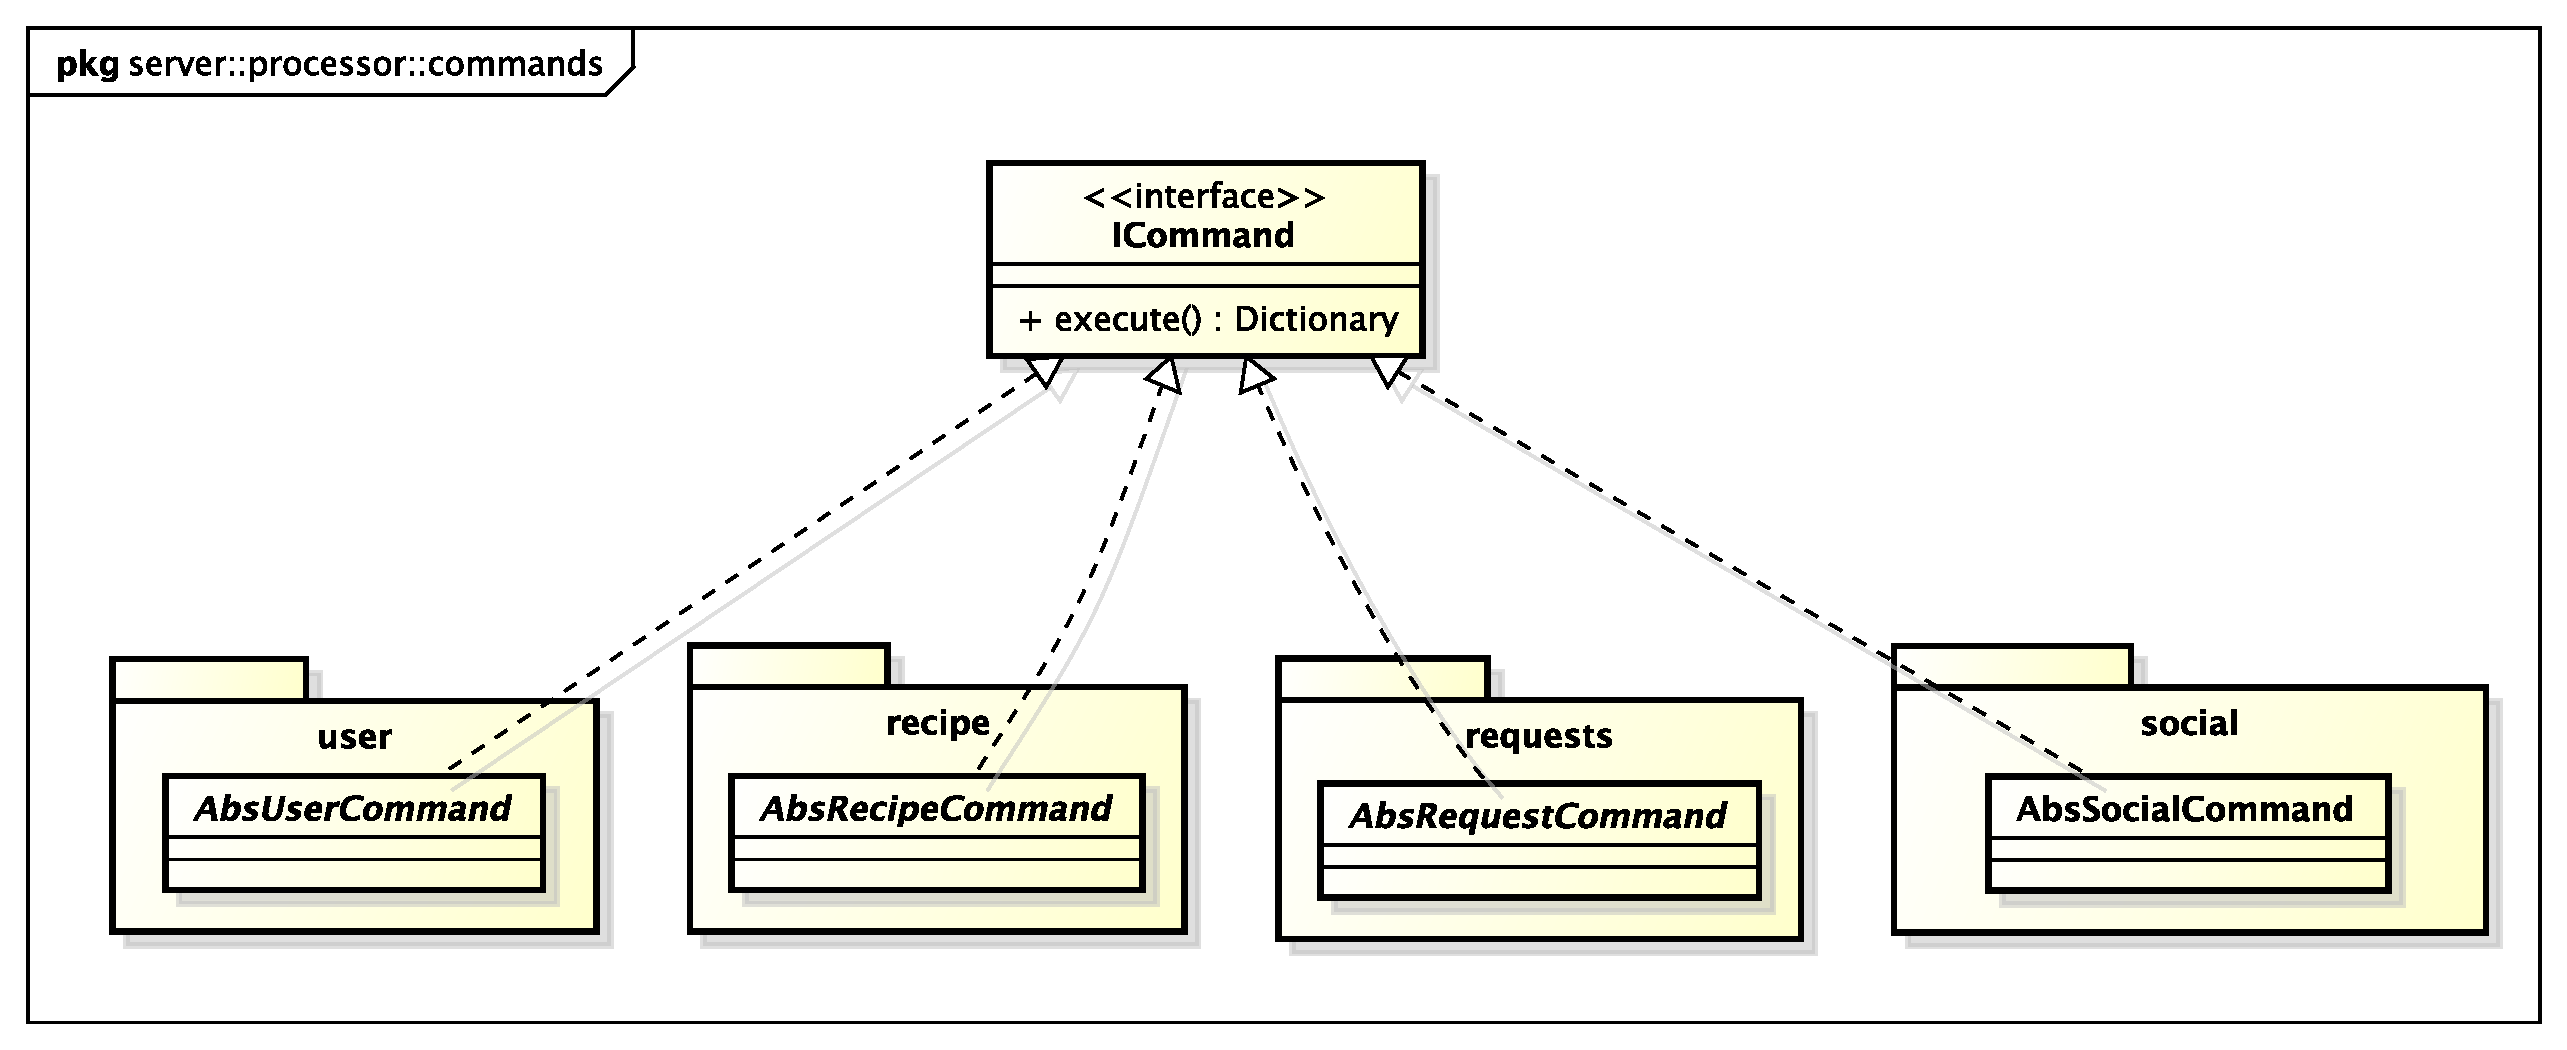
\includegraphics[scale=0.4]{./images/server/commands.pdf}}
      \caption{Package - server::processor::commands}
    \end{figure}
    \begin{itemize}
      \item \textbf{Descrizione}: contiene le classi ed i package che definiscono i diversi comandi contenenti la logica necessaria a soddisfare le varie richieste in arrivo dal client;
      \item \textbf{Padre}: server::processor
      \item \textbf{Package contenuti}:
        \begin{itemize}
          \item server::processor::commands::recipe
          \item server::processor::commands::requests
          \item server::processor::commands::user
          \item server::processor::commands::social
        \end{itemize}
      \item \textbf{Interazione con altri componenti}:
        \begin{itemize}
          \item server::db
        \end{itemize}
    \end{itemize}

      \paragraph{Classi} % (fold)

      \subparagraph{server::processor::commands::ICommand} % (fold)
      \label{subp:bdsm_app_server_processor_commands_icommand}
	    \begin{figure}[!htbp]
 	 		\centering
 			\centerline{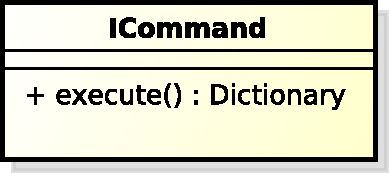
\includegraphics[scale=0.75]{./images/server/classes/processor/i_command.pdf}}
 			\caption{Classe - server::processor::ICommand}
		\end{figure}
      \begin{itemize}
        \item \textbf{Descrizione}: rappresenta un'interfaccia comune per tutti i comandi presenti nel package \texttt{server::commands} e figli;
        \item \textbf{Utilizzo}: espone un metodo \texttt{execute()}, il quale sarà implementato da tutti i comandi concreti;
    \item \textbf{Attributi}: N/A
    \item \textbf{Metodi}:
          \begin{itemize}
              \item \textcolor{forestgreen}{\texttt{+ execute(request: Dictionary) : Dictionary}}
              \begin{description}
                \item \textbf{Descrizione}: metodo astratto che definisce un contratto per tutte le classi che implementato ICommand. Accetta un parametro di tipo Dictionary, contente i dati della richiesta, e ritorna un oggetto dello stesso tipo contente i dati da ritornare alla chiamata (se necessari) ed informazioni successo o meno di esecuzione del comando.
              \end{description}
          \end{itemize}
      \end{itemize}
      % subparagraph bdsm_app::server_processor_abscommand (end)


      % ==============================
      % SERVER::COMMANDS::USER PACKAGE
      %
      \subsubsection{server::processor::commands::user} % (fold)
      \label{ssub:bdsm_app_server_processor_commands_user}
      \begin{figure}[!htbp]
        \centering
        \centerline{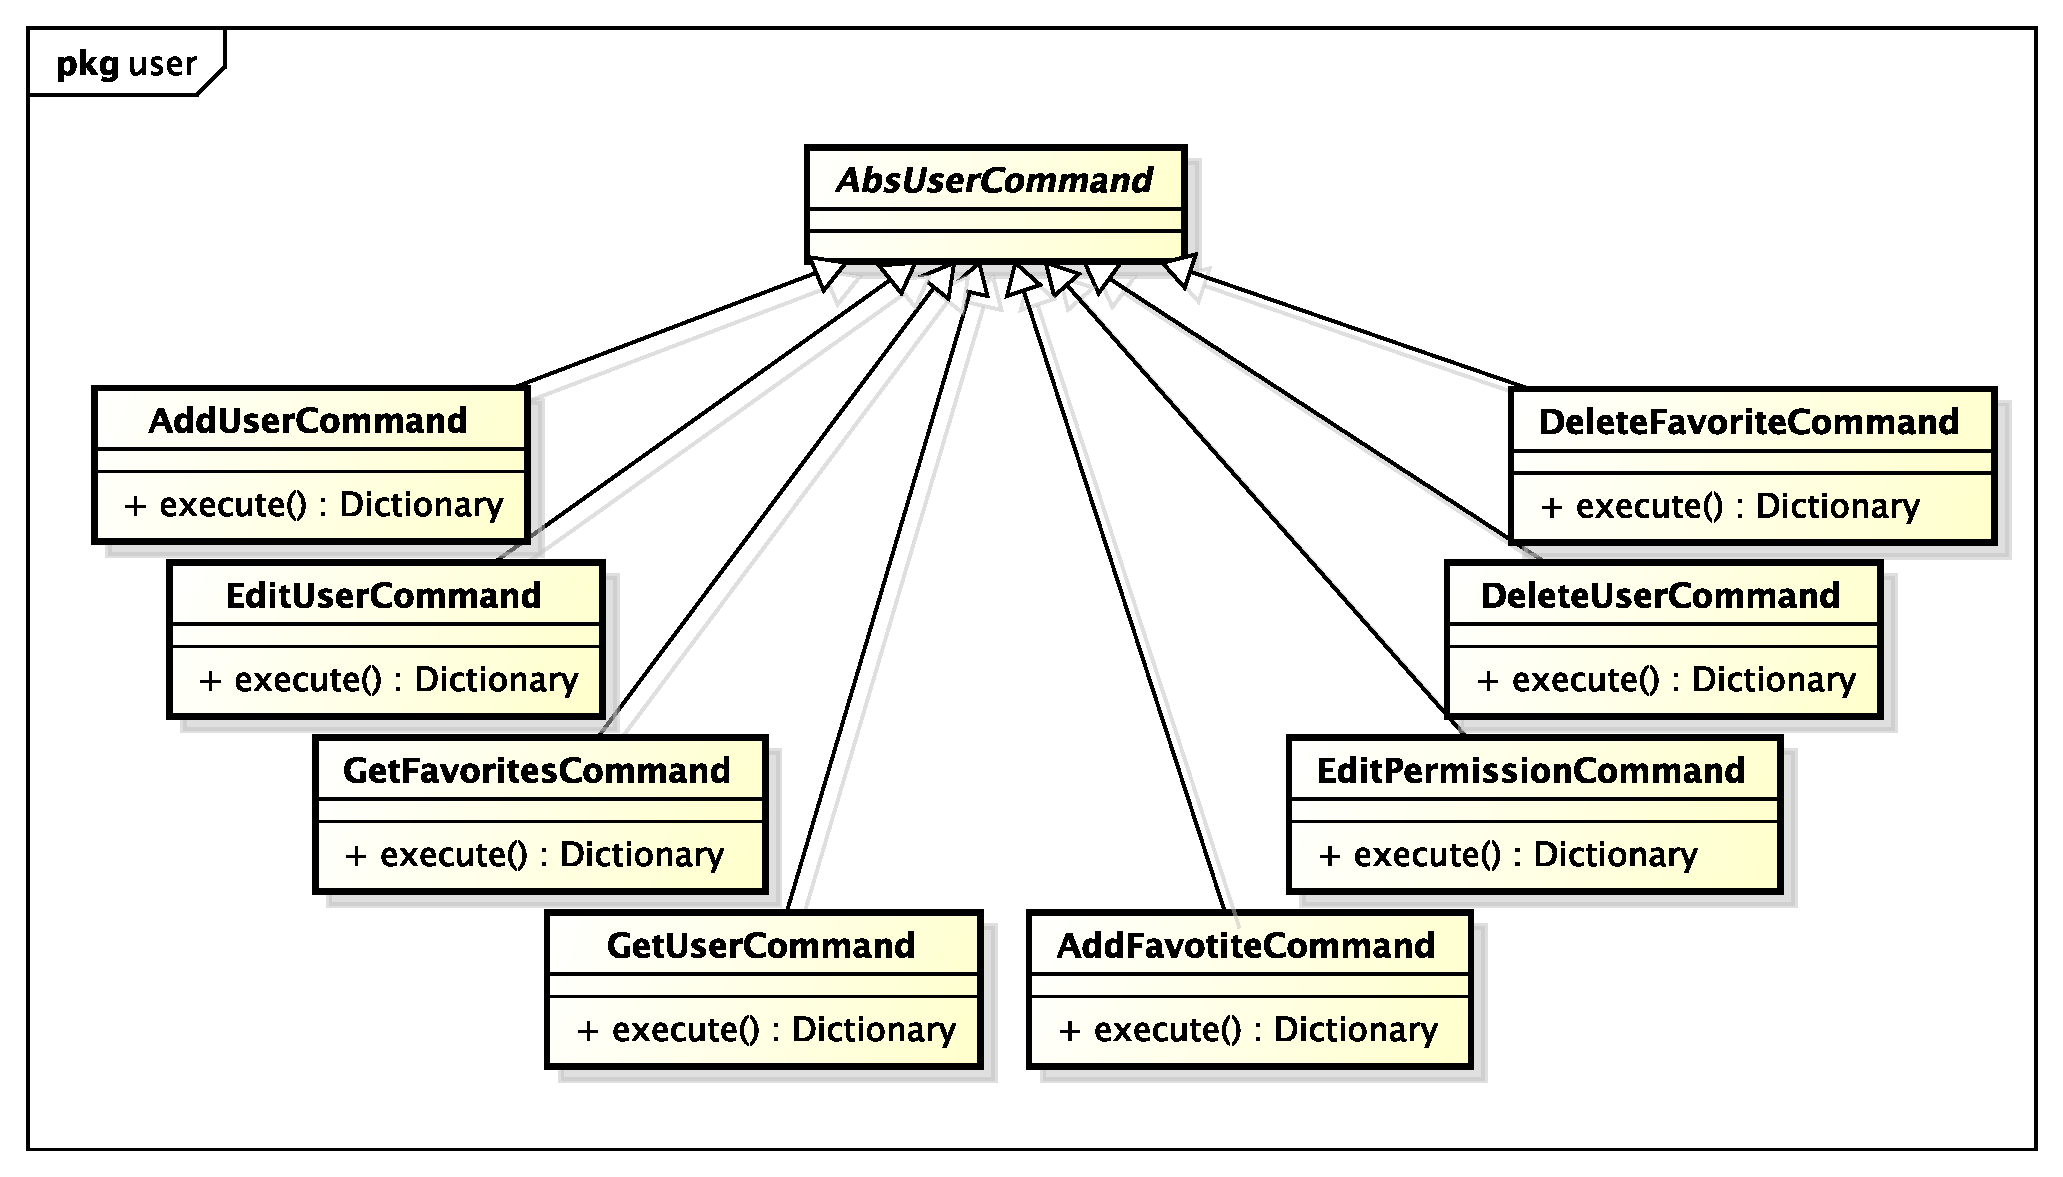
\includegraphics[scale=0.5]{./images/server/user.pdf}}
        \caption{Package - server::processor::commands::user}
      \end{figure}

      \begin{itemize}
        \item \textbf{Descrizione}: contiene tutti i comandi relativi alla gestione degli utenti;
        \item \textbf{Padre}: server::processor::commands;
        \item \textbf{Interazione con altri componenti}:
          \begin{itemize}
            \item server::db
          \end{itemize}
      \end{itemize}

        \paragraph{Classi} % (fold)

        \subparagraph{server::processor::commands::user::AbsUserCommand} % (fold)
        \label{subp:bdsm_app_server_processor_commands_user_absusercommand}
        \begin{itemize}
          \item \textbf{Descrizione}: rappresenta una classe comune a tutti i comandi relativi alla gestione degli utenti;
          \item \textbf{Utilizzo}: è stata rappresentata come classe in quanto potrà contenere uno o più metodi di utilità comuni a tutti i comandi relativi alla gestione degli utenti;
          \item \textbf{Relazioni con altre classi}:
            \begin{itemize}
              \item server::processor::commands::ICommand
            \end{itemize}
      \item \textbf{Attributi}: N/A
      \item \textbf{Metodi}: N/A
        \end{itemize}
        % subparagraph (end)

        \subparagraph{server::processor::commands::user::LoginCommand} % (fold)
        \label{subp:bdsm_app_server_processor_commands_user_LoginCommand}
        \begin{itemize}
          \item \textbf{Descrizione}: definisce la logica per effettuare il login al sistema;
          \item \textbf{Utilizzo}: implementa il metodo \texttt{execute()} che conterrà la logica per scambiare le informazioni di accesso al sistema;
          \item \textbf{Relazioni con altre classi}:
            \begin{itemize}
              \item server::processor::commands::user::AbsUserCommand
            \end{itemize}
          \item \textbf{Attributi}: N/A
          \item \textbf{Metodi}:
          \begin{itemize}
              \item \textcolor{forestgreen}{\texttt{+ execute(request: Dictionary) : Dictionary}}
              \begin{description}
                \item \textbf{Descrizione}: esegue l'accesso al sistema.
              \end{description}
          \end{itemize}
        \end{itemize}
        % subparagraph (end)

        \subparagraph{server::processor::commands::user::LogoutCommand} % (fold)
        \label{subp:bdsm_app_server_processor_commands_user_LogoutCommand}
        \begin{itemize}
          \item \textbf{Descrizione}: definisce la logica per effettuare la disconnessione dal sistema;
          \item \textbf{Utilizzo}: implementa il metodo \texttt{execute()} che conterrà la logica per effettuare l'operazione di logout dal sistema;
          \item \textbf{Relazioni con altre classi}:
            \begin{itemize}
              \item server::processor::commands::user::AbsUserCommand
            \end{itemize}
          \item \textbf{Attributi}: N/A
          \item \textbf{Metodi}:
          \begin{itemize}
              \item \textcolor{forestgreen}{\texttt{+ execute(request: Dictionary) : Dictionary}}
              \begin{description}
                \item \textbf{Descrizione}: esegue la disconnessione dal sistema.
              \end{description}
          \end{itemize}
        \end{itemize}
        % subparagraph (end)

        \subparagraph{server::processor::commands::user::AddUserCommand} % (fold)
        \label{subp:bdsm_app_server_processor_commands_user_addusercommand}
        \begin{itemize}
          \item \textbf{Descrizione}: definisce la logica per aggiungere un nuovo utente al database;
          \item \textbf{Utilizzo}: implementa il metodo \texttt{execute()} che conterrà la logica per aggiungere un nuovo utente al database;
          \item \textbf{Relazioni con altre classi}:
            \begin{itemize}
              \item server::processor::commands::user::AbsUserCommand
            \end{itemize}
          \item \textbf{Attributi}: N/A
          \item \textbf{Metodi}:
          \begin{itemize}
              \item \textcolor{forestgreen}{\texttt{+ execute(request: Dictionary) : Dictionary}}
              \begin{description}
                \item \textbf{Descrizione}: aggiunge un nuovo utente al database.
              \end{description}
          \end{itemize}
        \end{itemize}
        % subparagraph (end)

        \subparagraph{server::processor::commands::user::GetUserCommand} % (fold)
        \label{subp:bdsm_app_server_processor_commands_user_getusercommand}
        \begin{itemize}
          \item \textbf{Descrizione}: definisce la logica per ricavare un determinato utente dal database;
          \item \textbf{Utilizzo}: implementa il metodo \texttt{execute()} che conterrà la logica per ricavare un determinato utente dal database;
          \item \textbf{Relazioni con altre classi}:
            \begin{itemize}
              \item server::processor::commands::user::AbsUserCommand
            \end{itemize}
          \item \textbf{Attributi}: N/A
          \item \textbf{Metodi}:
          \begin{itemize}
              \item \textcolor{forestgreen}{\texttt{+ execute(request: Dictionary) : Dictionary}}
              \begin{description}
                \item \textbf{Descrizione}: ritorna un determinato utente presente nel database.
              \end{description}
          \end{itemize}
        \end{itemize}
        % subparagraph (end)

        \subparagraph{server::processor::commands::user::DeleteUserCommand} % (fold)
        \label{subp:bdsm_app_server_processor_commands_user_deleteusercommand}
        \begin{itemize}
          \item \textbf{Descrizione}: definisce la logica per rimuovere un determinato utente dal database;
          \item \textbf{Utilizzo}: implementa il metodo \texttt{execute()} che conterrà la logica per rimuovere un determinato utente dal database;
          \item \textbf{Relazioni con altre classi}:
            \begin{itemize}
              \item server::processor::commands::user::AbsUserCommand
            \end{itemize}
          \item \textbf{Attributi}: N/A
          \item \textbf{Metodi}:
          \begin{itemize}
              \item \textcolor{forestgreen}{\texttt{+ execute(request: Dictionary) : Dictionary}}
              \begin{description}
                \item \textbf{Descrizione}: elimina un determinato utente dal database.
              \end{description}
          \end{itemize}
        \end{itemize}
        % subparagraph (end)

        \subparagraph{server::processor::commands::user::EditUserCommand} % (fold)
        \label{subp:bdsm_app_server_processor_commands_user_editusercommand}
        \begin{itemize}
          \item \textbf{Descrizione}: definisce la logica per modificare i dati un determinato utente dal database;
          \item \textbf{Utilizzo}: implementa il metodo \texttt{execute()} che conterrà la logica per modificare i dati un determinato utente dal database;
          \item \textbf{Relazioni con altre classi}:
            \begin{itemize}
              \item server::processor::commands::user::AbsUserCommand
            \end{itemize}
          \item \textbf{Attributi}: N/A
          \item \textbf{Metodi}:
          \begin{itemize}
              \item \textcolor{forestgreen}{\texttt{+ execute(request: Dictionary) : Dictionary}}
              \begin{description}
                \item \textbf{Descrizione}: modifica i dati associati ad un determinato utente presente nel database.
              \end{description}
          \end{itemize}
        \end{itemize}
        % subparagraph (end)

        \subparagraph{server::processor::commands::user::EditPermissionCommand} % (fold)
        \label{subp:bdsm_app_server_processor_commands_user_editpermissioncommand}
        \begin{itemize}
          \item \textbf{Descrizione}: definisce la logica per modificare i permessi di un determinato utente;
          \item \textbf{Utilizzo}: implementa il metodo \texttt{execute()} che conterrà la logica per modificare i permessi di un determinato utente;
          \item \textbf{Relazioni con altre classi}:
            \begin{itemize}
              \item server::processor::commands::user::AbsUserCommand
            \end{itemize}
          \item \textbf{Attributi}: N/A
          \item \textbf{Metodi}:
          \begin{itemize}
              \item \textcolor{forestgreen}{\texttt{+ execute(request: Dictionary) : Dictionary}}
              \begin{description}
                \item \textbf{Descrizione}: modifica i permessi di un determinato utente presente nel database.
              \end{description}
          \end{itemize}
        \end{itemize}
        % subparagraph (end)

        \subparagraph{server::processor::commands::user::GetFavouritesCommand} % (fold)
        \label{subp:bdsm_app_server_processor_commands_user_getfavouritescommand}
        \begin{itemize}
          \item \textbf{Descrizione}: definisce la logica per ottenere le View preferite di un determinato utente;
          \item \textbf{Utilizzo}: implementa il metodo \texttt{execute()} che conterrà la logica per ottenere le View preferite di un determinato utente;
          \item \textbf{Relazioni con altre classi}:
            \begin{itemize}
              \item server::processor::commands::user::AbsUserCommand
            \end{itemize}
          \item \textbf{Attributi}: N/A
          \item \textbf{Metodi}:
          \begin{itemize}
              \item \textcolor{forestgreen}{\texttt{+ execute(request: Dictionary) : Dictionary}}
              \begin{description}
                \item \textbf{Descrizione}: ritorna i preferiti associati ad un determinato utente.
              \end{description}
          \end{itemize}
        \end{itemize}
        % subparagraph (end)

        \subparagraph{server::processor::commands::user::DeleteFavouriteCommand} % (fold)
        \label{subp:bdsm_app_server_processor_commands_user_deletefavouritecommand}
        \begin{itemize}
          \item \textbf{Descrizione}: definisce la logica per rimuovere un determinato preferito da un utente specifico;
          \item \textbf{Utilizzo}: implementa il metodo \texttt{execute()} che conterrà la logica per rimuovere un determinato preferito da un utente specifico;
          \item \textbf{Relazioni con altre classi}:
            \begin{itemize}
              \item server::processor::commands::user::AbsUserCommand
            \end{itemize}
          \item \textbf{Attributi}: N/A
          \item \textbf{Metodi}:
          \begin{itemize}
              \item \textcolor{forestgreen}{\texttt{+ execute(request: Dictionary) : Dictionary}}
              \begin{description}
                \item \textbf{Descrizione}: rimuove dal database un determinato preferito associato ad un utente.
              \end{description}
          \end{itemize}
        \end{itemize}
        % subparagraph (end)

        \subparagraph{server::processor::commands::user::AddFavouriteCommand} % (fold)
        \label{subp:bdsm_app_server_processor_commands_user_addfavouritecommand}
        \begin{itemize}
          \item \textbf{Descrizione}: definisce la logica per aggiungere un preferito ad un determinato utente;
          \item \textbf{Utilizzo}: implementa il metodo \texttt{execute()} che conterrà la logica per aggiungere un preferito ad un determinato utente;
          \item \textbf{Relazioni con altre classi}:
            \begin{itemize}
              \item server::processor::commands::user::AbsUserCommand
            \end{itemize}
          \item \textbf{Attributi}: N/A
          \item \textbf{Metodi}:
          \begin{itemize}
              \item \textcolor{forestgreen}{\texttt{+ execute(request: Dictionary) : Dictionary}}
              \begin{description}
                \item \textbf{Descrizione}: aggiunge al database un preferito associato ad un determinato utente.
              \end{description}
          \end{itemize}
        \end{itemize}
        % subparagraph (end)
      % subsection


      % ================================
      % SERVER::COMMANDS::RECIPE PACKAGE
      %
      \subsubsection{server::processor::commands::recipe} % (fold)
      \label{ssub:bdsm_app_server_processor_commands_recipe}
      \begin{figure}[!htbp]
        \centering
        \centerline{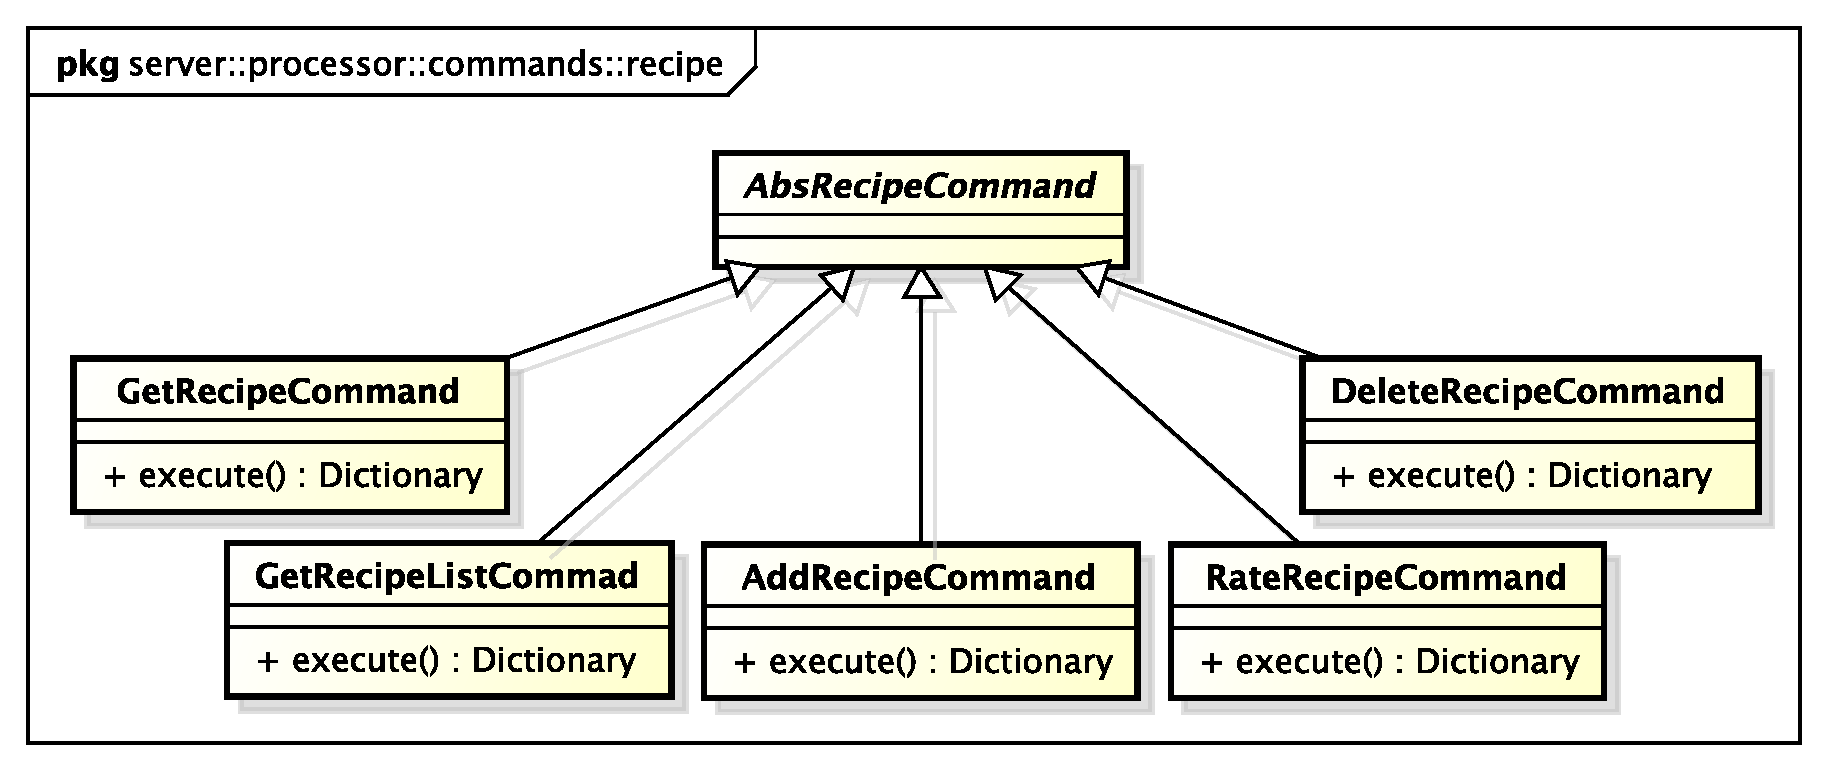
\includegraphics[scale=0.5]{./images/server/recipe.pdf}}
        \caption{Package - server::processor::commands::recipe}
      \end{figure}

      \begin{itemize}
        \item \textbf{Descrizione}: contiene tutti i comandi relativi alla gestione delle Recipe;
        \item \textbf{Padre}: server::commands
        \item \textbf{Interazione con altri componenti}:
          \begin{itemize}
            \item server::db
          \end{itemize}
      \end{itemize}

        \paragraph{Classi} % (fold)

        \subparagraph{server::processor::commands::recipe::AbsRecipeCommand} % (fold)
        \label{subp:bdsm_app_server_processor_commands_recipe_absrecipecommand}
        \begin{itemize}
          \item \textbf{Descrizione}: rappresenta una classe comune a tutti i comandi relativi alla gestione delle Recipe;
          \item \textbf{Utilizzo}: è stata rappresentata come classe in quanto potrà contenere uno o più metodi di utilità comuni a tutti i comandi relativi alla gestione delle Recipe;
          \item \textbf{Relazioni con altre classi}:
            \begin{itemize}
              \item server::processor::commands::ICommand;
            \end{itemize}
          \item \textbf{Attributi}: N/A
          \item \textbf{Metodi}: N/A
        \end{itemize}
        % subparagraph (end)

        \subparagraph{server::processor::commands::recipe::GetRecipeCommand} % (fold)
        \label{subp:bdsm_app_server_processor_commands_recipe_getrecipecommand}
        \begin{itemize}
          \item \textbf{Descrizione}: definisce la logica per ottenere una determinata Recipe e la lista delle metriche associata ad essa;
          \item \textbf{Utilizzo}: implementa il metodo \texttt{execute()} che conterrà la logica per ottenere una determinata Recipe e la lista delle metriche associata ad essa;
          \item \textbf{Relazioni con altre classi}:
            \begin{itemize}
              \item server::processor::commands::recipe::AbsRecipeCommand
            \end{itemize}
          \item \textbf{Attributi}: N/A
          \item \textbf{Metodi}:
          \begin{itemize}
              \item \textcolor{forestgreen}{\texttt{+ execute(request: Dictionary) : Dictionary}}
              \begin{description}
                \item \textbf{Descrizione}: restituisce i dati associati ad una determinata Recipe presente nel database.
              \end{description}
          \end{itemize}
        \end{itemize}
        % subparagraph (end)

        \subparagraph{server::processor::commands::recipe::GetRecipeListCommand} % (fold)
        \label{subp:bdsm_app_server_processor_commands_recipe_getrecipelistcommand}
        \begin{itemize}
          \item \textbf{Descrizione}: definisce la logica per ottenere la lista delle Recipe presenti nel sistema;
          \item \textbf{Utilizzo}: implementa il metodo \texttt{execute()} che conterrà la logica per ottenere la lista delle Recipe presenti nel sistema;
          \item \textbf{Relazioni con altre classi}:
            \begin{itemize}
              \item server::processor::commands::recipe::AbsRecipeCommand
            \end{itemize}
          \item \textbf{Attributi}: N/A
          \item \textbf{Metodi}:
          \begin{itemize}
              \item \textcolor{forestgreen}{\texttt{+ execute(request: Dictionary) : Dictionary}}
              \begin{description}
                \item \textbf{Descrizione}: restituisce la lista delle Recipe presenti nel database.
              \end{description}
          \end{itemize}
        \end{itemize}
        % subparagraph (end)

        \subparagraph{server::processor::commands::recipe::AddRecipeCommand} % (fold)
        \label{subp:bdsm_app_server_processor_commands_recipe_addrecipecommand}
        \begin{itemize}
          \item \textbf{Descrizione}: definisce la logica per aggiungere una nuova Recipe al database;
          \item \textbf{Utilizzo}: implementa il metodo \texttt{execute()} che conterrà la logica per aggiungere una nuova Recipe al database;
          \item \textbf{Relazioni con altre classi}:
            \begin{itemize}
              \item server::processor::commands::recipe::AbsRecipeCommand
            \end{itemize}
          \item \textbf{Attributi}: N/A
          \item \textbf{Metodi}:
          \begin{itemize}
              \item \textcolor{forestgreen}{\texttt{+ execute(request: Dictionary) : Dictionary}}
              \begin{description}
                \item \textbf{Descrizione}: aggiunge una nuova Recipe al database.
              \end{description}
          \end{itemize}
        \end{itemize}
        % subparagraph (end)

        \subparagraph{server::processor::commands::recipe::DeleteRecipeCommand} % (fold)
        \label{subp:bdsm_app_server_processor_commands_recipe_deleterecipecommand}
        \begin{itemize}
          \item \textbf{Descrizione}: definisce la logica per rimuovere una determinata Recipe dal database;
          \item \textbf{Utilizzo}: implementa il metodo \texttt{execute()} che conterrà la logica per rimuovere una determinata Recipe dal database;
          \item \textbf{Relazioni con altre classi}:
            \begin{itemize}
              \item server::processor::commands::recipe::AbsRecipeCommand
            \end{itemize}
          \item \textbf{Attributi}: N/A
          \item \textbf{Metodi}:
          \begin{itemize}
              \item \textcolor{forestgreen}{\texttt{+ execute(request: Dictionary) : Dictionary}}
              \begin{description}
                \item \textbf{Descrizione}: rimuove una determinata Recipe dal database.
              \end{description}
          \end{itemize}
        \end{itemize}
        % subparagraph (end)

        \subparagraph{server::processor::commands::recipe::RateRecipeCommand} % (fold)
        \label{subp:bdsm_app_server_processor_commands_recipe_raterecipecommand}
        \begin{itemize}
          \item \textbf{Descrizione}: definisce la logica per aggiungere e modificare il rating ad un determinata Recipe;
          \item \textbf{Utilizzo}: implementa il metodo \texttt{execute()} che conterrà la logica per aggiungere e modificare il rating ad un determinata Recipe;
          \item \textbf{Relazioni con altre classi}:
            \begin{itemize}
              \item server::processor::commands::recipe::AbsRecipeCommand
            \end{itemize}
          \item \textbf{Attributi}: N/A
          \item \textbf{Metodi}:
          \begin{itemize}
              \item \textcolor{forestgreen}{\texttt{+ execute(request: Dictionary) : Dictionary}}
              \begin{description}
                \item \textbf{Descrizione}: aggiunge o modifica il rating di una determinata Recipe.
              \end{description}
          \end{itemize}
        \end{itemize}
        % subparagraph (end)


      % ================================
      % SERVER::COMMANDS::REQUESTS PACKAGE
      %
      \subsubsection{server::processor::commands::requests} % (fold)
      \label{ssub:bdsm_app_server_processor_commands_requests}
      \begin{figure}[!htbp]
        \centering
        \centerline{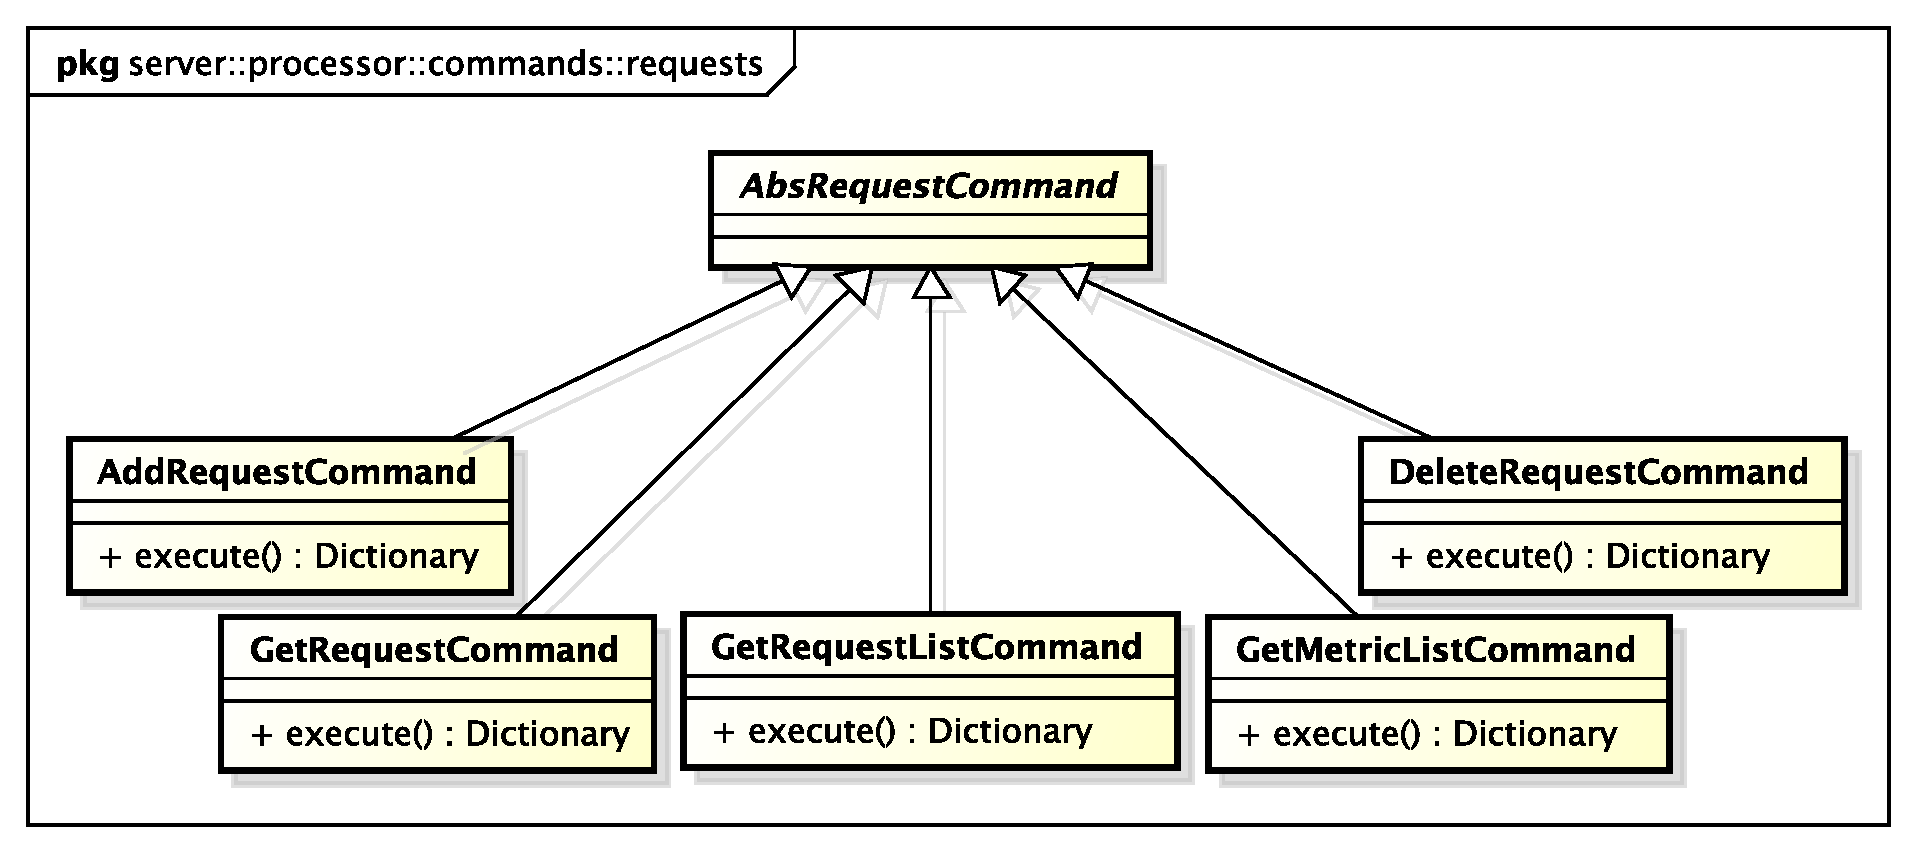
\includegraphics[scale=0.5]{./images/server/requests.pdf}}
        \caption{Package - server::processor::commands::requests}
      \end{figure}

      \begin{itemize}
        \item \textbf{Descrizione}: contiene tutti i comandi relativi alla gestione delle richieste di aggiunta Recipe;
        \item \textbf{Padre}: server::processor::commands;
        \item \textbf{Interazione con altri componenti}:
          \begin{itemize}
            \item server::db
          \end{itemize}
      \end{itemize}

        \paragraph{Classi} % (fold)

        \subparagraph{server::processor::commands::requests::AbsRequestCommand} % (fold)
        \label{subp:bdsm_app_server_processor_commands_requests_absrequestcommand}
        \begin{itemize}
          \item \textbf{Descrizione}: rappresenta una classe comune a tutti i comandi relativi alla gestione delle richieste di aggiunta Recipe;
          \item \textbf{Utilizzo}: è stata rappresentata come classe in quanto potrà contenere uno o più metodi di utilità comuni a tutti i comandi relativi alla gestione delle richieste di aggiunta Recipe;
          \item \textbf{Relazioni con altre classi}:
            \begin{itemize}
              \item server::processor::commands::ICommand
            \end{itemize}
          \item \textbf{Attributi}: N/A
          \item \textbf{Metodi}: N/A
        \end{itemize}
        % subparagraph (end)

        \subparagraph{server::processor::commands::requests::GetRequestCommand} % (fold)
        \label{subp:bdsm_app_server_processor_commands_requests_getrequestcommand}
        \begin{itemize}
          \item \textbf{Descrizione}: definisce la logica per ottenere un determinata richiesta di aggiunta Recipe dal database;
          \item \textbf{Utilizzo}: implementa il metodo \texttt{execute()} che conterrà la logica per ottenere una determinata richiesta di aggiunta Recipe dal database;
          \item \textbf{Relazioni con altre classi}:
            \begin{itemize}
              \item server::processor::commands::requests::AbsRequestCommand
            \end{itemize}
          \item \textbf{Attributi}: N/A
          \item \textbf{Metodi}:
          \begin{itemize}
              \item \textcolor{forestgreen}{\texttt{+ execute(request: Dictionary) : Dictionary}}
              \begin{description}
                \item \textbf{Descrizione}: restituisce i dati associati ad una determinata richiesta di aggiunta Recipe presente nel database.
              \end{description}
          \end{itemize}
        \end{itemize}
        % subparagraph (end)

        \subparagraph{server::processor::commands::requests::AddRequestCommand} % (fold)
        \label{subp:bdsm_app_server_processor_commands_requests_addrequestcommand}
        \begin{itemize}
          \item \textbf{Descrizione}: definisce la logica per aggiungere una nuova richiesta di aggiunta Recipe al database;
          \item \textbf{Utilizzo}: implementa il metodo \texttt{execute()} che conterrà la logica per aggiungere una nuova richiesta di aggiunta Recipe al database;
          \item \textbf{Relazioni con altre classi}:
            \begin{itemize}
              \item server::processor::commands::requests::AbsRequestCommand
            \end{itemize}
          \item \textbf{Attributi}: N/A
          \item \textbf{Metodi}:
          \begin{itemize}
              \item \textcolor{forestgreen}{\texttt{+ execute(request: Dictionary) : Dictionary}}
              \begin{description}
                \item \textbf{Descrizione}: aggiunge una nuova richiesta di aggiunta Recipe al database.
              \end{description}
          \end{itemize}
        \end{itemize}
        % subparagraph (end)

        \subparagraph{server::processor::commands::requests::GetRequestListCommand} % (fold)
        \label{subp:bdsm_app_server_processor_commands_requests_getrequestlistcommand}
        \begin{itemize}
          \item \textbf{Descrizione}: definisce la logica per ottenere la lista delle richieste di aggiunta Recipe presenti nel database;
          \item \textbf{Utilizzo}: implementa il metodo \texttt{execute()} che conterrà la logica per ottenere la lista delle richieste di aggiunta Recipe presenti nel database;
          \item \textbf{Relazioni con altre classi}:
            \begin{itemize}
              \item server::processor::commands::requests::AbsRequestCommand
            \end{itemize}
          \item \textbf{Attributi}: N/A
          \item \textbf{Metodi}:
          \begin{itemize}
              \item \textcolor{forestgreen}{\texttt{+ execute(request: Dictionary) : Dictionary}}
              \begin{description}
                \item \textbf{Descrizione}: restituisce i dati associati ad una determinata richiesta di aggiunta Recipe presente nel database.
              \end{description}
          \end{itemize}
        \end{itemize}
        % subparagraph (end)

        \subparagraph{server::processor::commands::requests::DeleteRequestCommand} % (fold)
        \label{subp:bdsm_app_server_processor_commands_requests_deleterequestcommand}
        \begin{itemize}
          \item \textbf{Descrizione}: definisce la logica per rimuovere una determinata richiesta di aggiunta Recipe dal database;
          \item \textbf{Utilizzo}: implementa il metodo \texttt{execute()} che conterrà la logica per rimuovere una determinata richiesta di aggiunta Recipe dal database;
          \item \textbf{Relazioni con altre classi}:
            \begin{itemize}
              \item server::processor::commands::requests::AbsRequestCommand
            \end{itemize}
          \item \textbf{Attributi}: N/A
          \item \textbf{Metodi}:
          \begin{itemize}
              \item \textcolor{forestgreen}{\texttt{+ execute(request: Dictionary) : Dictionary}}
              \begin{description}
                \item \textbf{Descrizione}: rimuove una determinata richiesta di aggiunta Recipe presente nel database.
              \end{description}
          \end{itemize}
        \end{itemize}
        % subparagraph (end)

        \subparagraph{server::processor::commands::requests::GetMetricsListCommand} % (fold)
        \label{subp:bdsm_app_server_processor_commands_requests_getmetricslistcommand}
        \begin{itemize}
          \item \textbf{Descrizione}: definisce la logica per ottenere la lista delle metriche presenti in una determinata richiesta di aggiunta Recipe;
          \item \textbf{Utilizzo}: implementa il metodo \texttt{execute()} che conterrà la logica per ottenere la lista delle metriche presenti in una determinata richiesta di aggiunta Recipe;
          \item \textbf{Relazioni con altre classi}:
            \begin{itemize}
              \item server::processor::commands::requests::AbsRequestCommand
            \end{itemize}
          \item \textbf{Attributi}: N/A
          \item \textbf{Metodi}:
          \begin{itemize}
              \item \textcolor{forestgreen}{\texttt{+ execute(request: Dictionary) : Dictionary}}
              \begin{description}
                \item \textbf{Descrizione}: restituisce la lista delle metriche associate ad una determinata Recipe.
              \end{description}
          \end{itemize}
        \end{itemize}
        % subparagraph (end)

        % ================================
      % SERVER::COMMANDS::SOCIAL PACKAGE
      %
      \subsubsection{server::processor::commands::social} % (fold)
      \label{ssub:bdsm_app_server_processor_commands_social}
      \begin{figure}[!htbp]
        \centering
        \centerline{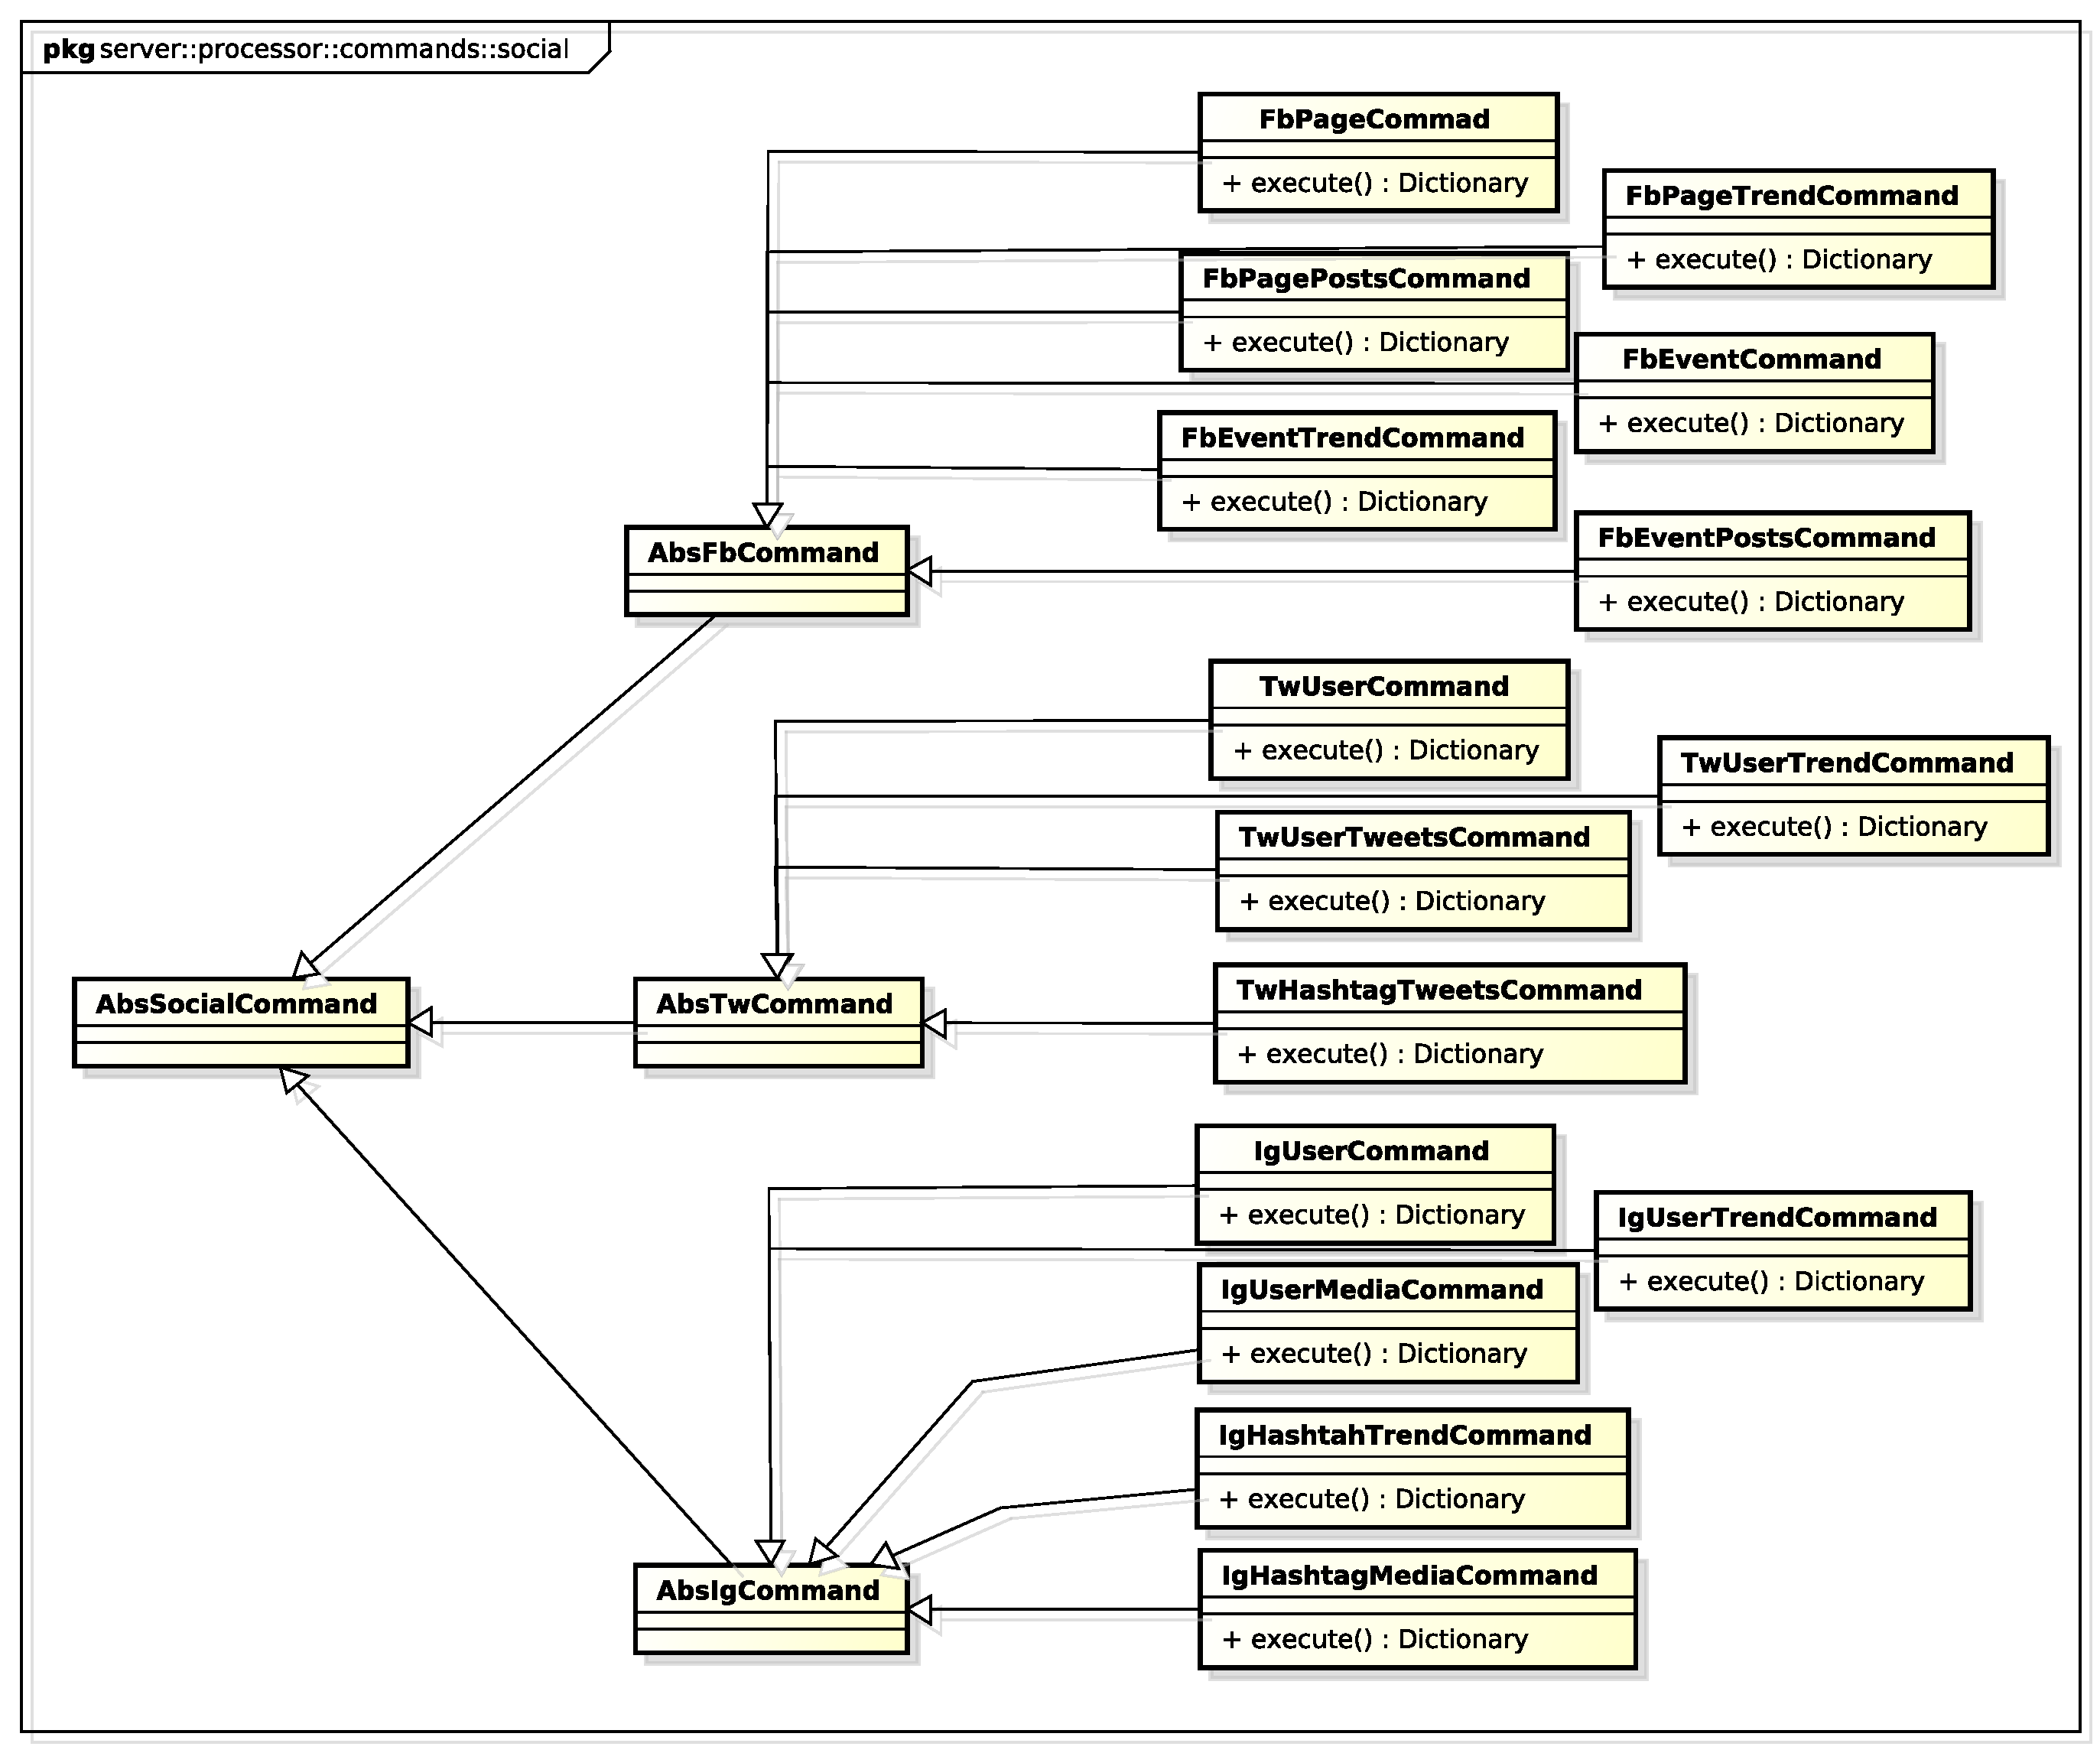
\includegraphics[scale=0.4]{./images/server/social.pdf}}
        \caption{Package - server::processor::commands::social}
      \end{figure}

      \begin{itemize}
        \item \textbf{Descrizione}: contiene tutti i comandi che per ottenere tutti i dati grezzi ricavati dai social network;
        \item \textbf{Padre}: server::processor::commands;
        \item \textbf{Interazione con altri componenti}:
          \begin{itemize}
            \item server::db
          \end{itemize}
      \end{itemize}

        \paragraph{Classi} % (fold)

        \subparagraph{server::processor::commands::social::AbsSocialCommand} % (fold)
        \label{subp:bdsm_app_server_processor_commands_social_abssocialcommand}
        \begin{itemize}
          \item \textbf{Descrizione}: rappresenta una classe comune a tutti i comandi relativi alla gestione dei dati grezzi ricavati dai social network;
          \item \textbf{Utilizzo}: è stata rappresentata come classe in quanto potrà contenere uno o più metodi di utilità comuni a tutti i comandi relativi alla gestione dei dati grezzi ricavati dai social network;
          \item \textbf{Relazioni con altre classi}:
            \begin{itemize}
              \item server::processor::commands::ICommand
            \end{itemize}
          \item \textbf{Attributi}: N/A
          \item \textbf{Metodi}: N/A
        \end{itemize}
        % subparagraph (end)

        % FACEBOOK

        \subparagraph{server::processor::commands::social::AbsFbCommand} % (fold)
        \label{subp:bdsm_app_server_processor_commands_social_absfbcommand}
        \begin{itemize}
          \item \textbf{Descrizione}: rappresenta una classe comune a tutti i comandi relativi alla gestione dei dati grezzi ricavati da Facebook;
          \item \textbf{Utilizzo}: è stata rappresentata come classe in quanto potrà contenere uno o più metodi di utilità comuni a tutti i comandi relativi alla gestione dei dati grezzi ricavati da Facebook;
          \item \textbf{Relazioni con altre classi}:
            \begin{itemize}
              \item server::processor::commands::social::AbsSocialCommand
            \end{itemize}
          \item \textbf{Attributi}: N/A
          \item \textbf{Metodi}: N/A
        \end{itemize}
        % subparagraph (end)

        \subparagraph{server::processor::commands::social::FbPageCommand} % (fold)
        \label{subp:bdsm_app_server_processor_commands_social_fbpagecommand}
        \begin{itemize}
          \item \textbf{Descrizione}: definisce la logica per ottenere i dati grezzi relativi ad una pagina Facebook;
          \item \textbf{Utilizzo}: implementa il metodo \texttt{execute()} che conterrà la logica per ottenere i dati grezzi relativi ad una pagina Facebook;
          \item \textbf{Relazioni con altre classi}:
            \begin{itemize}
              \item server::processor::commands::social::AbsFbCommand
            \end{itemize}
          \item \textbf{Attributi}: N/A
          \item \textbf{Metodi}:
          \begin{itemize}
              \item \textcolor{forestgreen}{\texttt{+ execute(request: Dictionary) : Dictionary}}
              \begin{description}
                \item \textbf{Descrizione}: restituisce i dati associati ad una determinata pagina Facebook presente nel database.
              \end{description}
          \end{itemize}
        \end{itemize}
        % subparagraph (end)

        \subparagraph{server::processor::commands::social::FbPageTrendCommand} % (fold)
        \label{subp:bdsm_app_server_processor_commands_social_fbpagetrendcommand}
        \begin{itemize}
          \item \textbf{Descrizione}: definisce la logica per ottenere i dati grezzi relativi al trend di una pagina Facebook;
          \item \textbf{Utilizzo}: implementa il metodo \texttt{execute()} che conterrà la logica per ottenere i dati grezzi relativi al trend di una pagina Facebook;
          \item \textbf{Relazioni con altre classi}:
            \begin{itemize}
              \item server::processor::commands::social::AbsFbCommand
            \end{itemize}
          \item \textbf{Attributi}: N/A
          \item \textbf{Metodi}:
          \begin{itemize}
              \item \textcolor{forestgreen}{\texttt{+ execute(request: Dictionary) : Dictionary}}
              \begin{description}
                \item \textbf{Descrizione}: restituisce i dati associati al trend di una determinata pagina Facebook presente nel database.
              \end{description}
          \end{itemize}
        \end{itemize}
        % subparagraph (end)

        \subparagraph{server::processor::commands::social::FbPageEventCommand} % (fold)
        \label{subp:bdsm_app_server_processor_commands_social_fbpageeventcommand}
        \begin{itemize}
          \item \textbf{Descrizione}: definisce la logica per ottenere i dati relativi a tutti gli eventi associati ad una pagina Facebook;
          \item \textbf{Utilizzo}: implementa il metodo \texttt{execute()} che conterrà la logica per ottenere i dati relativi a tutti gli eventi associati ad una pagina Facebook;
          \item \textbf{Relazioni con altre classi}:
            \begin{itemize}
              \item server::processor::commands::social::AbsFbCommand
            \end{itemize}
          \item \textbf{Attributi}: N/A
          \item \textbf{Metodi}:
          \begin{itemize}
              \item \textcolor{forestgreen}{\texttt{+ execute(request: Dictionary) : Dictionary}}
              \begin{description}
                \item \textbf{Descrizione}: restituisce i dati associati a tutti gli eventi di una determinata pagina Facebook presente nel database.
              \end{description}
          \end{itemize}
        \end{itemize}
        % subparagraph (end)

        \subparagraph{server::processor::commands::social::FbEventCommand} % (fold)
        \label{subp:bdsm_app_server_processor_commands_social_fbeventcommand}
        \begin{itemize}
          \item \textbf{Descrizione}: definisce la logica per ottenere i dati grezzi relativi ad un evento Facebook;
          \item \textbf{Utilizzo}: implementa il metodo \texttt{execute()} che conterrà la logica per ottenere i dati grezzi relativi ad un evento Facebook;
          \item \textbf{Relazioni con altre classi}:
            \begin{itemize}
              \item server::processor::commands::social::AbsFbCommand
            \end{itemize}
            \item \textbf{Attributi}: N/A
            \item \textbf{Metodi}:
            \begin{itemize}
                \item \textcolor{forestgreen}{\texttt{+ execute(request: Dictionary) : Dictionary}}
                \begin{description}
                  \item \textbf{Descrizione}: restituisce i dati associati ad un determinato evento Facebook presente nel database.
                \end{description}
            \end{itemize}
        \end{itemize}
        % subparagraph (end)

        \subparagraph{server::processor::commands::social::FbEventTrendCommand} % (fold)
        \label{subp:bdsm_app_server_processor_commands_social_fbeventtrendcommand}
        \begin{itemize}
          \item \textbf{Descrizione}: definisce la logica per ottenere i dati grezzi relativi al trend di un evento Facebook;
          \item \textbf{Utilizzo}: implementa il metodo \texttt{execute()} che conterrà la logica per ottenere i dati grezzi relativi al trend di un evento Facebook;
          \item \textbf{Relazioni con altre classi}:
            \begin{itemize}
              \item server::processor::commands::social::AbsFbCommand
            \end{itemize}
            \item \textbf{Attributi}: N/A
            \item \textbf{Metodi}:
            \begin{itemize}
                \item \textcolor{forestgreen}{\texttt{+ execute(request: Dictionary) : Dictionary}}
                \begin{description}
                  \item \textbf{Descrizione}: restituisce i dati associati al trend di un determinato evento Facebook presente nel database.
                \end{description}
            \end{itemize}
        \end{itemize}
        % subparagraph (end)

        \subparagraph{server::processor::commands::social::FbEventPostCommand} % (fold)
        \label{subp:bdsm_app_server_processor_commands_social_fbeventpostcommand}
        \begin{itemize}
          \item \textbf{Descrizione}: definisce la logica per ottenere i dati grezzi relativi al trend dei post di un evento Facebook;
          \item \textbf{Utilizzo}: implementa il metodo \texttt{execute()} che conterrà la logica per ottenere i dati grezzi relativi al trend dei post di un evento Facebook;
          \item \textbf{Relazioni con altre classi}:
            \begin{itemize}
              \item server::processor::commands::social::AbsFbCommand
            \end{itemize}
            \item \textbf{Attributi}: N/A
            \item \textbf{Metodi}:
            \begin{itemize}
                \item \textcolor{forestgreen}{\texttt{+ execute(request: Dictionary) : Dictionary}}
                \begin{description}
                  \item \textbf{Descrizione}: restituisce i dati associati al trend dei post di un determinato avento Facebook presente nel database.
                \end{description}
            \end{itemize}
        \end{itemize}
        % subparagraph (end)

        % TWITTER

        \subparagraph{server::processor::commands::social::AbsTwCommand} % (fold)
        \label{subp:bdsm_app_server_processor_commands_social::abstwcommand}
        \begin{itemize}
          \item \textbf{Descrizione}: rappresenta una classe comune a tutti i comandi relativi alla gestione dei dati grezzi ricavati da Twitter;
          \item \textbf{Utilizzo}: è stata rappresentata come classe in quanto potrà contenere uno o più metodi di utilità comuni a tutti i comandi relativi alla gestione dei dati grezzi ricavati da Twitter;
          \item \textbf{Relazioni con altre classi}:
            \begin{itemize}
              \item server::processor::commands::social::AbsSocialCommand
            \end{itemize}
          \item \textbf{Attributi}: N/A
          \item \textbf{Metodi}: N/A
        \end{itemize}
        % subparagraph (end)

        \subparagraph{server::processor::commands::social::TwUserCommand} % (fold)
        \label{subp:bdsm_app_server_processor_commands_social_twusercommand}
        \begin{itemize}
          \item \textbf{Descrizione}: definisce la logica per ottenere i dati grezzi relativi ad un utente Twitter;
          \item \textbf{Utilizzo}: implementa il metodo \texttt{execute()} che conterrà la logica per ottenere i dati grezzi relativi ad un utente Twitter;
          \item \textbf{Relazioni con altre classi}:
            \begin{itemize}
              \item server::processor::commands::social::AbsTwCommand
            \end{itemize}
          \item \textbf{Attributi}: N/A
          \item \textbf{Metodi}:
          \begin{itemize}
              \item \textcolor{forestgreen}{\texttt{+ execute(request: Dictionary) : Dictionary}}
              \begin{description}
                \item \textbf{Descrizione}: restituisce i dati associati ad un determinato utente Twitter presente nel database.
              \end{description}
          \end{itemize}
        \end{itemize}
        % subparagraph (end)

        \subparagraph{server::processor::commands::social::TwUserTrendCommand} % (fold)
        \label{subp:bdsm_app_server_processor_commands_social_twusertrendcommand}
        \begin{itemize}
          \item \textbf{Descrizione}: definisce la logica per ottenere i dati grezzi relativi al trend di un utente Twitter;
          \item \textbf{Utilizzo}: implementa il metodo \texttt{execute()} che conterrà la logica per ottenere i dati grezzi relativi al trend di un utente Twitter;
          \item \textbf{Relazioni con altre classi}:
            \begin{itemize}
              \item server::processor::commands::social::AbsTwCommand
            \end{itemize}
          \item \textbf{Attributi}: N/A
          \item \textbf{Metodi}:
          \begin{itemize}
              \item \textcolor{forestgreen}{\texttt{+ execute(request: Dictionary) : Dictionary}}
              \begin{description}
                \item \textbf{Descrizione}: restituisce i dati associati al trend di un determinato utente Twitter presente nel database.
              \end{description}
          \end{itemize}
        \end{itemize}
        % subparagraph (end)

        \subparagraph{server::processor::commands::social::TwUserTweetsCommand} % (fold)
        \label{subp:bdsm_app_server_processor_commands_social_twcommand}
        \begin{itemize}
          \item \textbf{Descrizione}: definisce la logica per ottenere i dati grezzi relativi al trend dei tweet di un utente Twitter;
          \item \textbf{Utilizzo}: implementa il metodo \texttt{execute()} che conterrà la logica per ottenere i dati grezzi relativi al trend dei tweet di un utente Twitter;
          \item \textbf{Relazioni con altre classi}:
            \begin{itemize}
              \item server::processor::commands::social::AbsTwCommand
            \end{itemize}
          \item \textbf{Attributi}: N/A
          \item \textbf{Metodi}:
          \begin{itemize}
              \item \textcolor{forestgreen}{\texttt{+ execute(request: Dictionary) : Dictionary}}
              \begin{description}
                \item \textbf{Descrizione}: restituisce i dati associati al trend dei tweet di un determinato utente Twitter presente nel database.
              \end{description}
          \end{itemize}
        \end{itemize}
        % subparagraph (end)

        \subparagraph{server::processor::commands::social::TwHashtagTweetsCommand} % (fold)
        \label{subp:bdsm_app_server_processor_commands_social_twhashtagtweetscommand}
        \begin{itemize}
          \item \textbf{Descrizione}: definisce la logica per ottenere i dati grezzi associati al trend dei tweet relativi ad un determinato hashtag;
          \item \textbf{Utilizzo}: implementa il metodo \texttt{execute()} che conterrà la logica per ottenere i dati grezzi associati al trend dei tweet relativi ad un determinato hashtag;
          \item \textbf{Relazioni con altre classi}:
            \begin{itemize}
              \item server::processor::commands::social::AbsTwCommand
            \end{itemize}
          \item \textbf{Attributi}: N/A
          \item \textbf{Metodi}:
          \begin{itemize}
              \item \textcolor{forestgreen}{\texttt{+ execute(request: Dictionary) : Dictionary}}
              \begin{description}
                \item \textbf{Descrizione}: restituisce i dati associati al trend dei tweet relativi ad un determinato hashtag Twitter presente nel database.
              \end{description}
          \end{itemize}
        \end{itemize}
        % subparagraph (end)

        % INSTAGRAM

        \subparagraph{server::processor::commands::social::AbsIgCommand} % (fold)
        \label{subp:bdsm_app_server_processor_commands_social_absigcommand}
        \begin{itemize}
          \item \textbf{Descrizione}: rappresenta una classe comune a tutti i comandi relativi alla gestione dei dati grezzi ricavati da Instagram;
          \item \textbf{Utilizzo}: è stata rappresentata come classe in quanto potrà contenere uno o più metodi di utilità comuni a tutti i comandi relativi alla gestione dei dati grezzi ricavati da Instagram;
          \item \textbf{Relazioni con altre classi}:
            \begin{itemize}
              \item server::processor::commands::social::AbsSocialCommand
            \end{itemize}
					\item \textbf{Attributi}: N/A
					\item \textbf{Metodi}: N/A
        \end{itemize}
        % subparagraph (end)

        \subparagraph{server::processor::commands::social::IgUserCommand} % (fold)
        \label{subp:bdsm_app_server_processor_commands_social_igusercommand}
        \begin{itemize}
          \item \textbf{Descrizione}: definisce la logica per ottenere i dati grezzi relativi ad un utente Instagram;
          \item \textbf{Utilizzo}: implementa il metodo \texttt{execute()} che conterrà la logica per ottenere i dati grezzi relativi ad un utente Instagram;
          \item \textbf{Relazioni con altre classi}:
            \begin{itemize}
              \item server::processor::commands::social::AbsIgCommand
            \end{itemize}
					\item \textbf{Attributi}: N/A
					\item \textbf{Metodi}:
        	\begin{itemize}
          		\item \textcolor{forestgreen}{\texttt{+ execute(request: Dictionary) : Dictionary}}
							\begin{description}
								\item \textbf{Descrizione}: restituisce i dati associati ad un determinato utente Instagram presente nel database.
							\end{description}
        	\end{itemize}
        \end{itemize}
        % subparagraph (end)

        \subparagraph{server::processor::commands::social::IgUserTrendCommand} % (fold)
        \label{subp:bdsm_app_server_processor_commands_social_igusertrendcommand}
        \begin{itemize}
          \item \textbf{Descrizione}: definisce la logica per ottenere i dati grezzi relativi al trend di un utente Instagram;
          \item \textbf{Utilizzo}: implementa il metodo \texttt{execute()} che conterrà la logica per ottenere i dati grezzi relativi al trend di un utente Instagram;
          \item \textbf{Relazioni con altre classi}:
            \begin{itemize}
              \item server::processor::commands::social::AbsIgCommand
            \end{itemize}
					\item \textbf{Attributi}: N/A
					\item \textbf{Metodi}:
        	\begin{itemize}
          		\item \textcolor{forestgreen}{\texttt{+ execute(request: Dictionary) : Dictionary}}
							\begin{description}
								\item \textbf{Descrizione}: restituisce i dati associati al trend di un determinato utente Instagram presente nel database.
							\end{description}
        	\end{itemize}
        \end{itemize}
        % subparagraph (end)

        \subparagraph{server::processor::commands::social::IgUserMediaCommand} % (fold)
        \label{subp:bdsm_app_server_processor_commands_social_igusermediacommand}
        \begin{itemize}
          \item \textbf{Descrizione}: definisce la logica per ottenere i dati grezzi relativi al trend dei media di un utente Instagram;
          \item \textbf{Utilizzo}: implementa il metodo \texttt{execute()} che conterrà la logica per ottenere i dati grezzi relativi al trend dei media di un utente Instagram;
          \item \textbf{Relazioni con altre classi}:
            \begin{itemize}
              \item server::processor::commands::social::AbsIgCommand
            \end{itemize}
					\item \textbf{Attributi}: N/A
					\item \textbf{Metodi}:
        	\begin{itemize}
          		\item \textcolor{forestgreen}{\texttt{+ execute(request: Dictionary) : Dictionary}}
							\begin{description}
								\item \textbf{Descrizione}: restituisce i dati associati al trend dei media di un determinato utente Instagram presente nel database.
							\end{description}
        	\end{itemize}
        \end{itemize}
        % subparagraph (end)

        \subparagraph{server::processor::commands::social::IgHashtagTrendCommand} % (fold)
        \label{subp:bdsm_app_server_processor_commands_social_ighashtagtrendcommand}
        \begin{itemize}
          \item \textbf{Descrizione}: definisce la logica per ottenere i dati grezzi relativi al trend di un hashtag di Instagram;
          \item \textbf{Utilizzo}: implementa il metodo \texttt{execute()} che conterrà la logica per ottenere i dati grezzi relativi al trend di un hashtag di Instagram;
          \item \textbf{Relazioni con altre classi}:
            \begin{itemize}
              \item server::processor::commands::social::AbsIgCommand
            \end{itemize}
					\item \textbf{Attributi}: N/A
				\item \textbf{Metodi}:
        	\begin{itemize}
          		\item \textcolor{forestgreen}{\texttt{+ execute(request: Dictionary) : Dictionary}}
							\begin{description}
								\item \textbf{Descrizione}: restituisce i dati associati al trend relativo ad un determinato hashtag Instagram presente nel database.
							\end{description}
        	\end{itemize}
        \end{itemize}
        % subparagraph (end)

        \subparagraph{server::processor::commands::social::IgHashtagMediaCommand} % (fold)
        \label{subp:bdsm_app_server_processor_commands_social_twhashtagmediacommand}
        \begin{itemize}
          \item \textbf{Descrizione}: definisce la logica per ottenere i dati grezzi relativi al trend dei media associati ad un hashtag di Instagram;
          \item \textbf{Utilizzo}: implementa il metodo \texttt{execute()} che conterrà la logica per ottenere i dati grezzi relativi al trend dei media associati ad un hashtag di Instagram;
          \item \textbf{Relazioni con altre classi}:
            \begin{itemize}
              \item server::processor::commands::social::AbsIgCommand
            \end{itemize}
					\item \textbf{Attributi}: N/A
				\item \textbf{Metodi}:
        	\begin{itemize}
          		\item \textcolor{forestgreen}{\texttt{+ execute(request: Dictionary) : Dictionary}}
							\begin{description}
								\item \textbf{Descrizione}: restituisce i dati associati al trend relativo ad un determinato hashtag Instagram presente nel database.
							\end{description}
        	\end{itemize}
        \end{itemize}
        % subparagraph (end)

    % subsubsection
  % subsubsection
% subsubsection
